%!TEX TS-program = xelatex
\documentclass{beamer}

\usepackage{BSU-theme/beamerthemeBSU} % Подгружаем тему

%%% Работа с русским языком и шрифтами
\usepackage[english,russian]{babel}   % загружает пакет многоязыковой вёрстки
\usepackage{fontspec}      % подготавливает загрузку шрифтов Open Type, True Type и др.
\defaultfontfeatures{Ligatures={TeX},Renderer=Basic}  % свойства шрифтов по умолчанию
\setmainfont[Ligatures={TeX,Historic}]{Arial} %TODO: Helvetica Light Normal
\setsansfont{Arial}  %TODO: Helvetica Light Normal
\setmonofont{Courier New}
\uselanguage{russian}
\languagepath{russian}
\deftranslation[to=russian]{Theorem}{Теорема}
\deftranslation[to=russian]{Definition}{Определение}
\deftranslation[to=russian]{Definitions}{Определения}
\deftranslation[to=russian]{Corollary}{Следствие}
\deftranslation[to=russian]{Fact}{Факт}
\deftranslation[to=russian]{Example}{Пример}
\deftranslation[to=russian]{Examples}{Примеры}

\usepackage{multicol}       % Несколько колонок
%\graphicspath{{images/}}    % Папка с картинками

\newcommand{\inp}[1]{\input{../../out/#1}}
\newcommand{\characteristic}[2]{\inp{#1/characteristics/#2}}
\newcommand{\descriptive}[2]{\inp{#1/descriptive/#2}}
\newcommand{\test}[3]{\inp{#1/test/#2/#3}}
\newcommand{\normaldistr}{$\mathcal{N}(\descriptive{original}{mean}, \descriptive{original}{variance})$}
\newcommand{\resnormaldistr}{$\mathcal{N}(\descriptive{residual}{mean}, \descriptive{residual}{variance})$}

%%% Информация об авторе и выступлении
\title[Анализ и прогнозирование гидрологических данных]{Анализ и прогнозирование гидрологических данных} 
\subtitle{Дипломная работа}
\author[Павлов А.С.]{Александр Сергеевич Павлов \\ \smallskip Научный руководитель: Цеховая Татьяна Вячеславовна}
\institute[БГУ, ФПМИ]{Факультет прикладной математики и информатики \\ \smallskip Кафедра теории вероятностей и математической статистики}
\date{Минск, \the\year}

\begin{document}    % Начало презентации

\frame[plain]{\titlepage}    % Титульный слайд

\section[Содержание]{}
\begin{frame}
  \frametitle{Содержание}
  \tableofcontents
\end{frame}

\section{Постановка задачи}
\begin{frame}
  \frametitle{Постановка задачи}
  \begin{enumerate}
    \item Предварительный статистический анализ гидроэкологических данных озера Баторино;
    \item Вариограммный анализ временного ряда: построение оценок семивариограммы,  подбор моделей семивариограммы;
    \item Исследование статистических свойств оценки семивариограммы гауссовского случайного процесса;
    \item Прогнозирование значений временного ряда с помощью интерполяционного метода Кригинг;
    \item Исследование точности прогноза в зависимости от оценки семивариограммы и модели семивариограммы, лежащих в основе метода Кригинг.
  \end{enumerate}
\end{frame}

\section{Обзор реализованного программного обеспечения}
\begin{frame}
  \frametitle{Обзор реализованного программного обеспечения}
  \framesubtitle{Особенности}
  \begin{itemize}
    \item Доступно с любого устройства, имеющего доступ в Интернет, по адресу \href{https://apaulau.shinyapps.io/batorino}{apaulau.shinyapps.io/batorino};
    \item Реализовано на языке программирования \textbf{R};
    \item Логически разделено на три модуля;
    \item Имеет простой, быстро расширяемый гибкий интерфейс;
    \item Широкие графические возможности;
    \item Проверка тестов и критериев;
    \item Мгновенный отклик на изменение параметров;
    \item Быстрая проверка различных моделей.
  \end{itemize}
\end{frame}

\subsection{Модуль предварительного анализа}
\begin{frame}
  \frametitle{Модуль предварительного анализа}
  \framesubtitle{Первичный анализ и описательные статистики}
  \begin{center}
    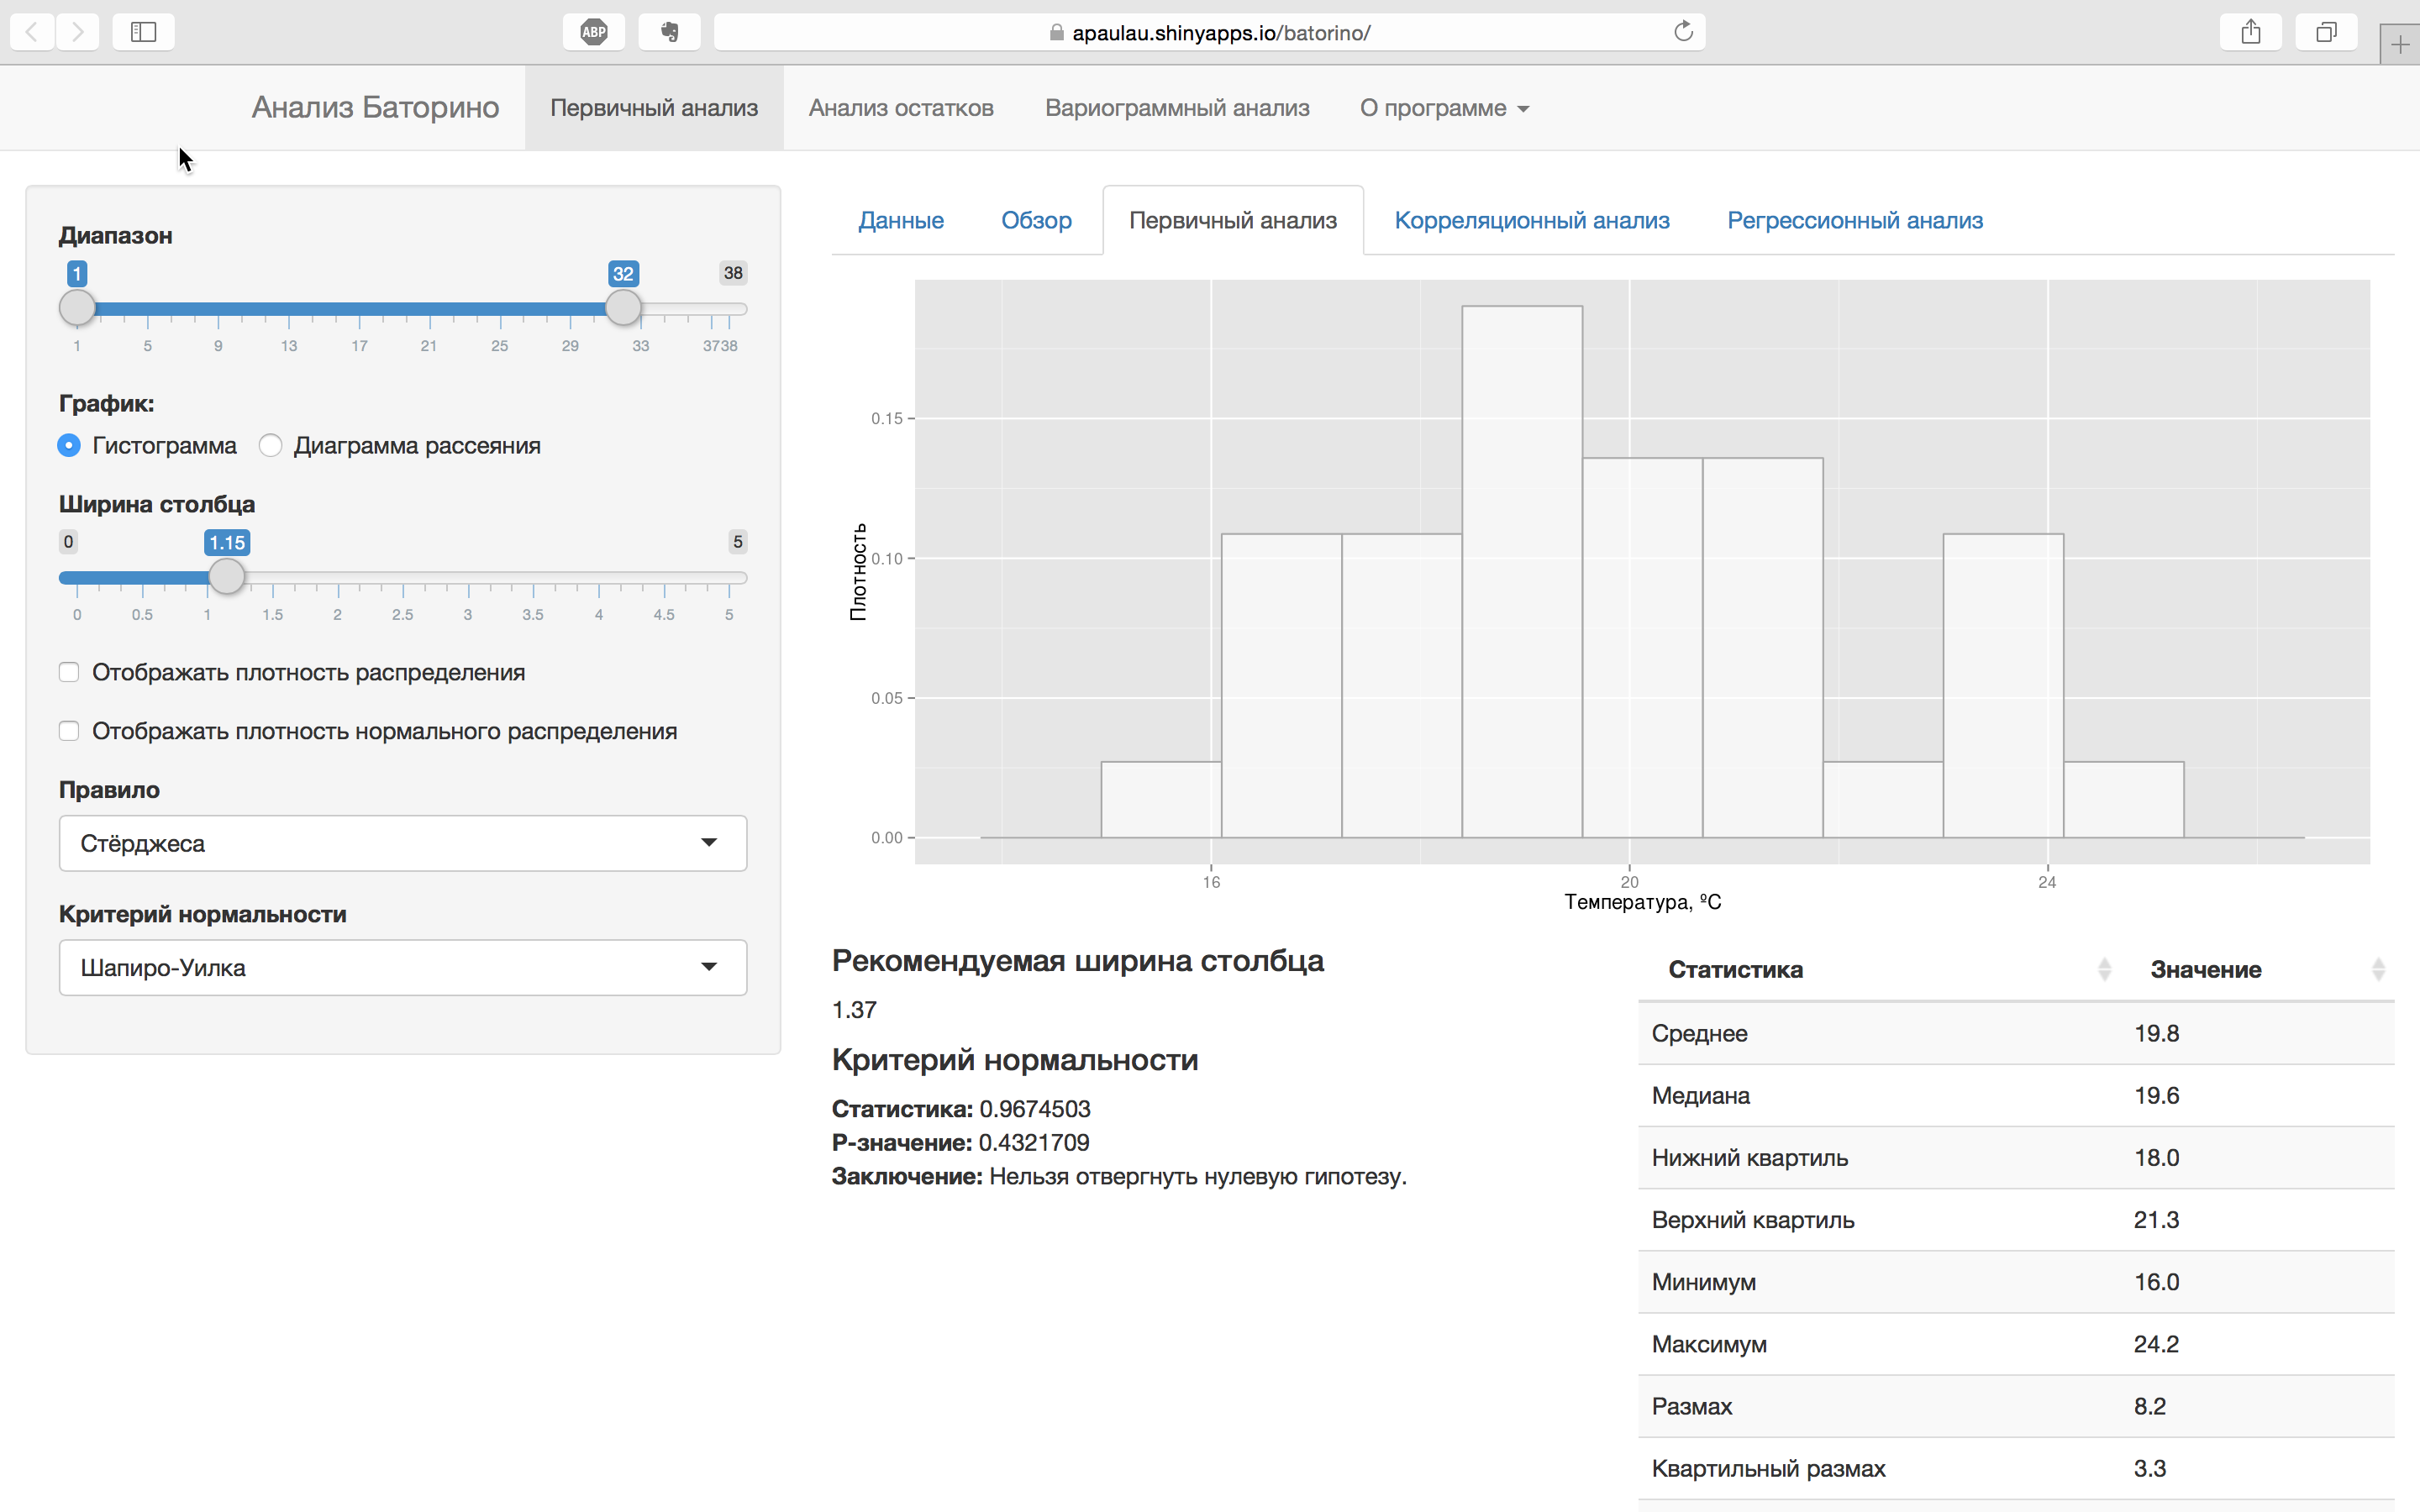
\includegraphics[width=0.9\textwidth]{../../figures/static/1_basis.png}
  \end{center}
\end{frame}

\begin{frame}
  \frametitle{Модуль предварительного анализа}
  \framesubtitle{Корреляционный анализ}
  \begin{center}
    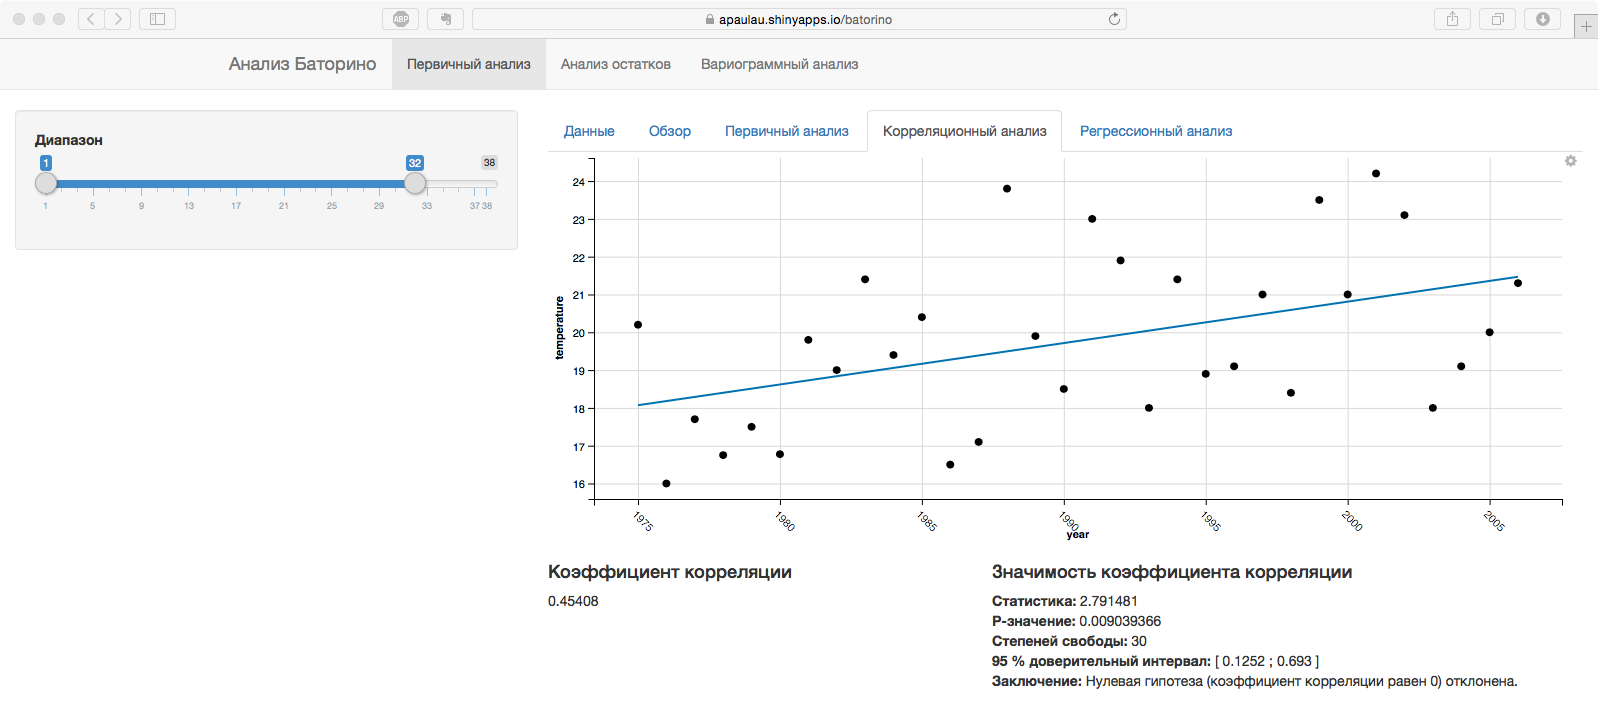
\includegraphics[width=0.9\textwidth]{../../figures/static/p_corr.png}
  \end{center}
\end{frame}

\begin{frame}
  \frametitle{Модуль предварительного анализа}
  \framesubtitle{Регрессионный анализ}
  \begin{center}
    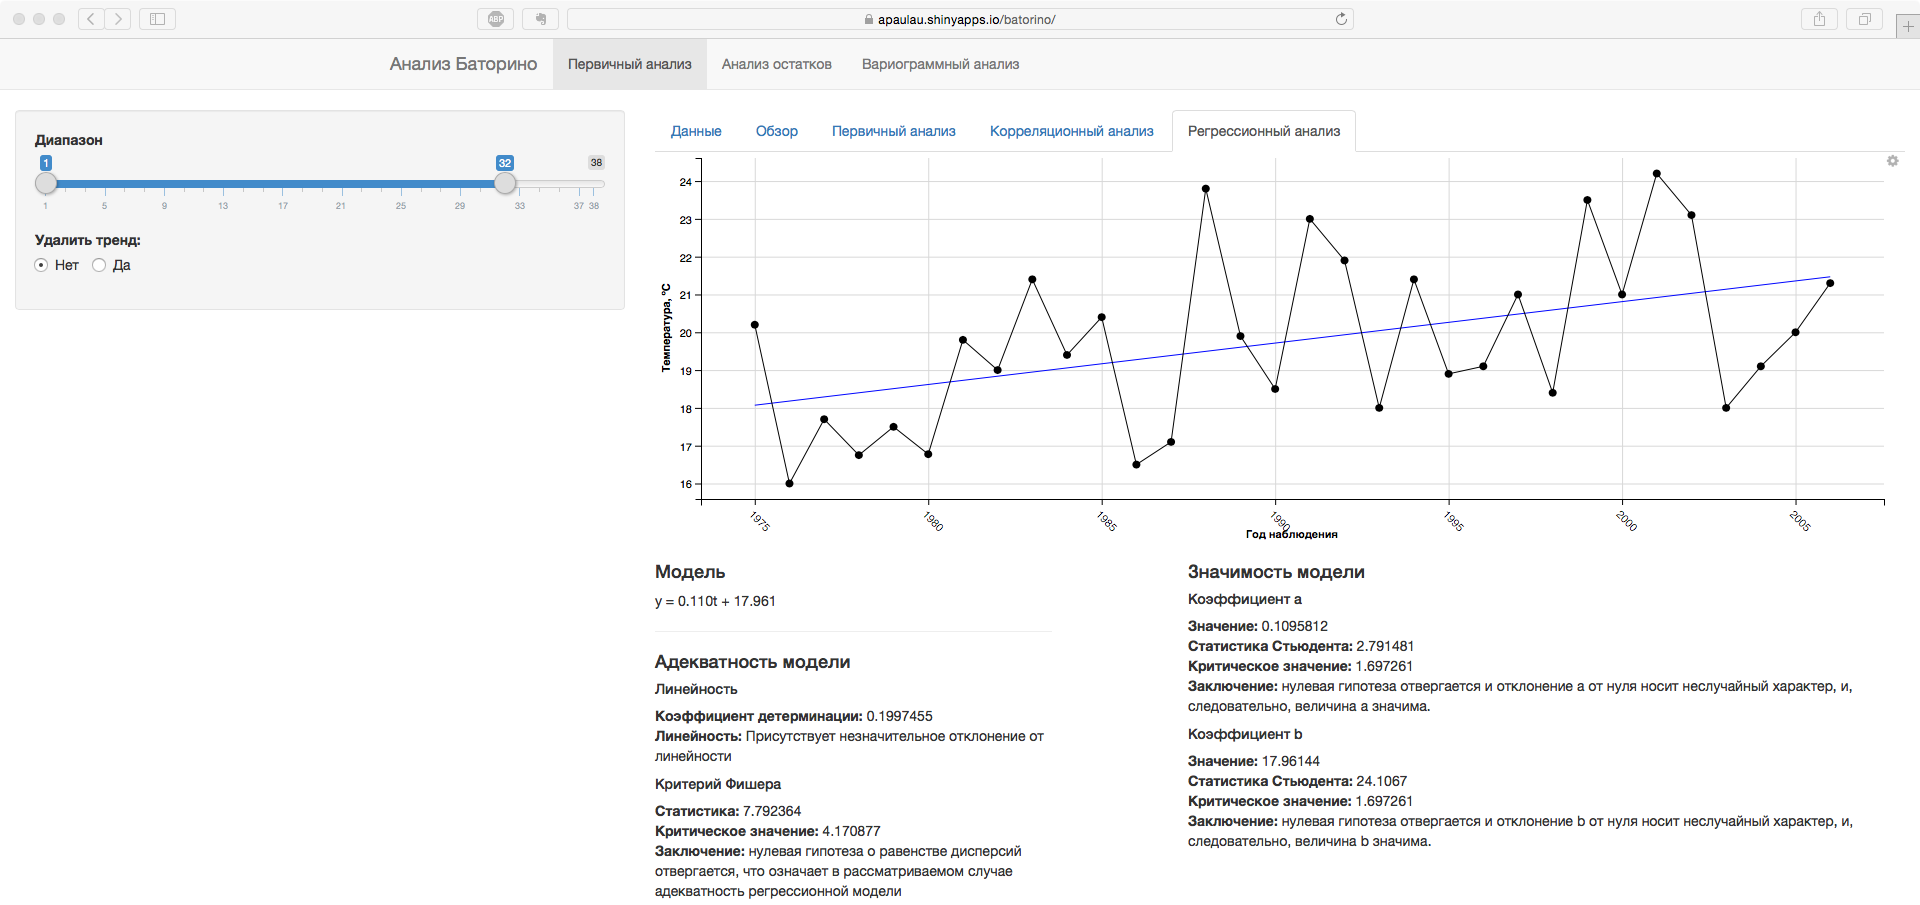
\includegraphics[width=0.9\textwidth]{../../figures/static/2_regr.png}
  \end{center}
\end{frame}

\subsection{Модуль анализа остатков}
\begin{frame}
  \frametitle{Модуль анализа остатков}
  \framesubtitle{Автокорреляционная функция}
  \begin{center}
    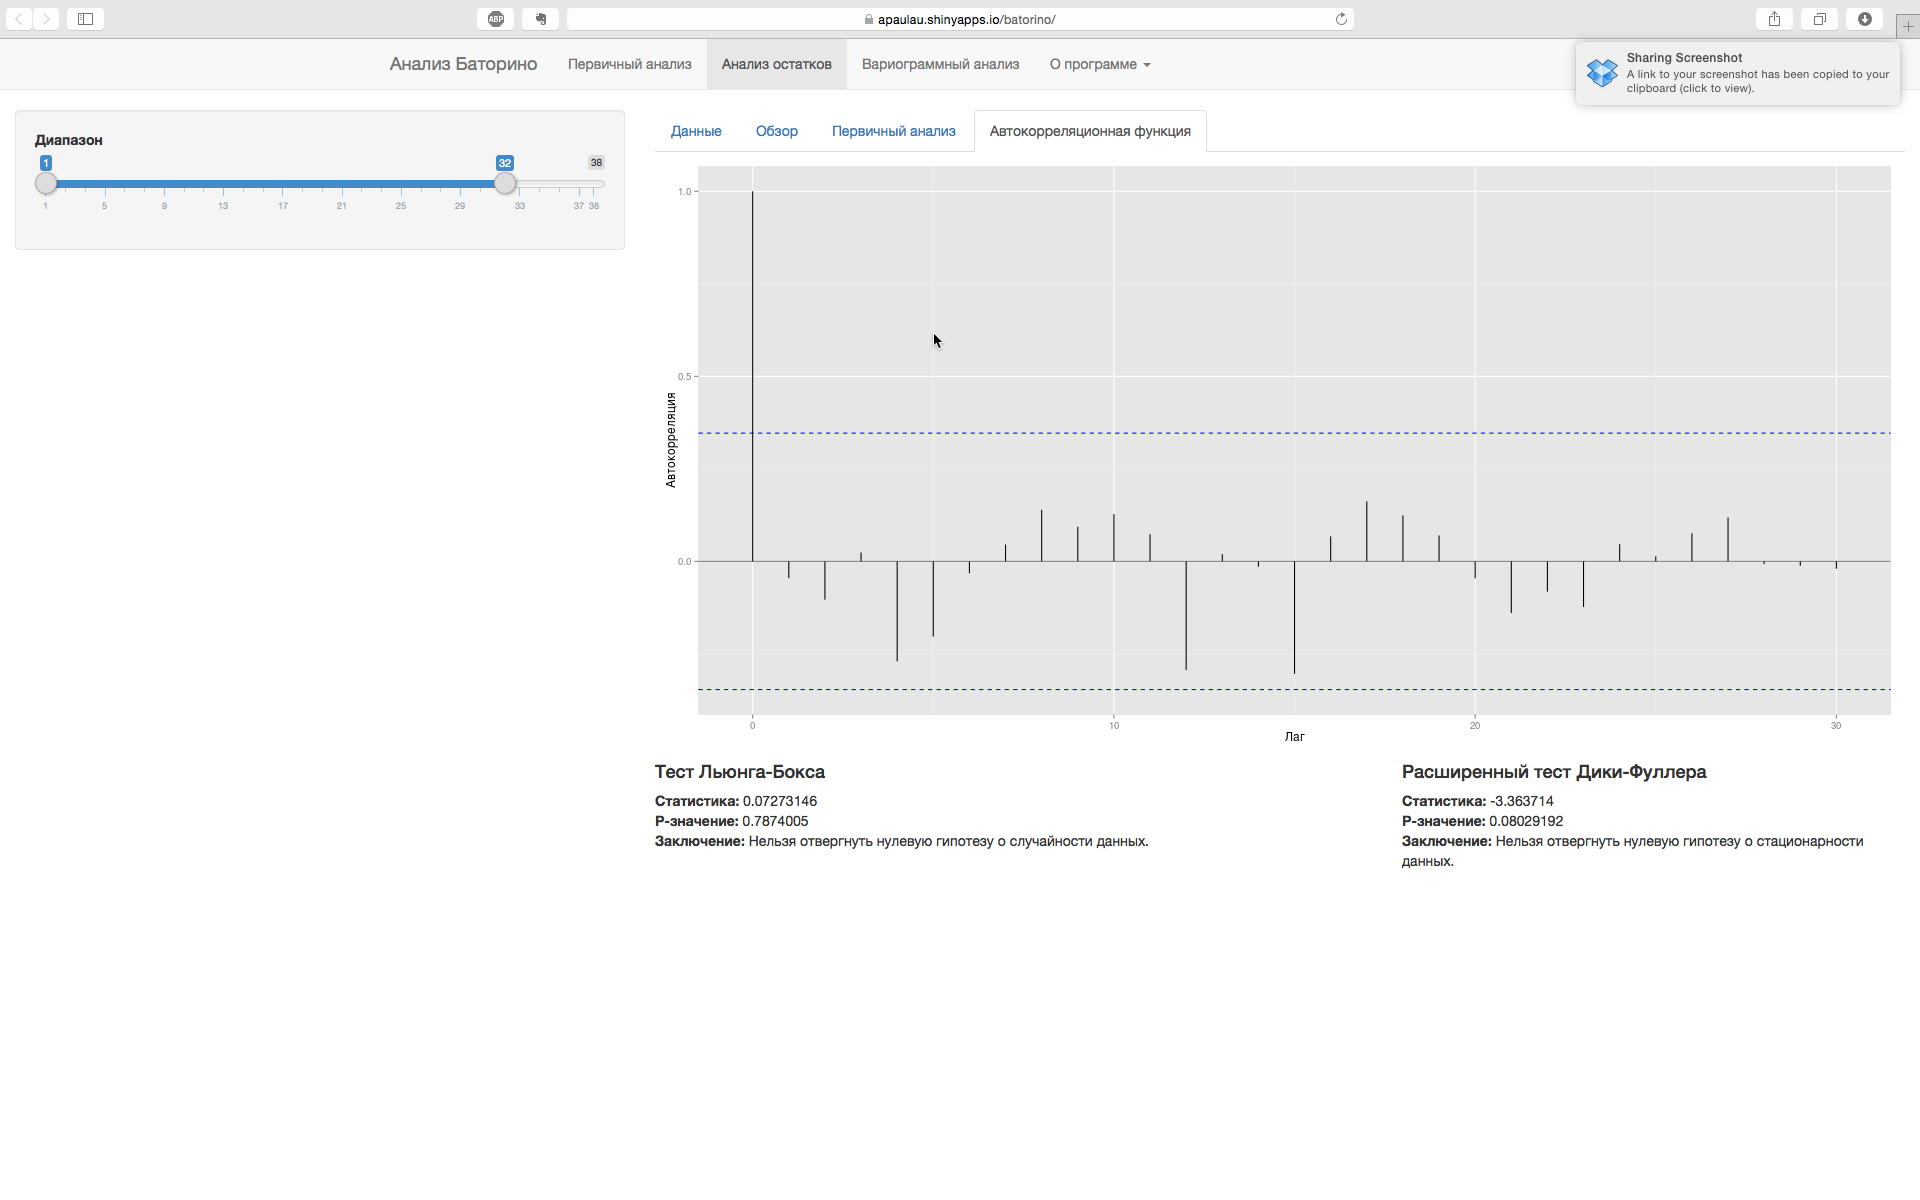
\includegraphics[width=0.9\textwidth]{../../figures/static/3_acf.png}
  \end{center}
\end{frame}

\subsection{Модуль вариограммного анализа}
\begin{frame}
  \frametitle{Модуль вариограммного анализа}
  \framesubtitle{Возможности по подбору модели вариограммы}
  \begin{center}
    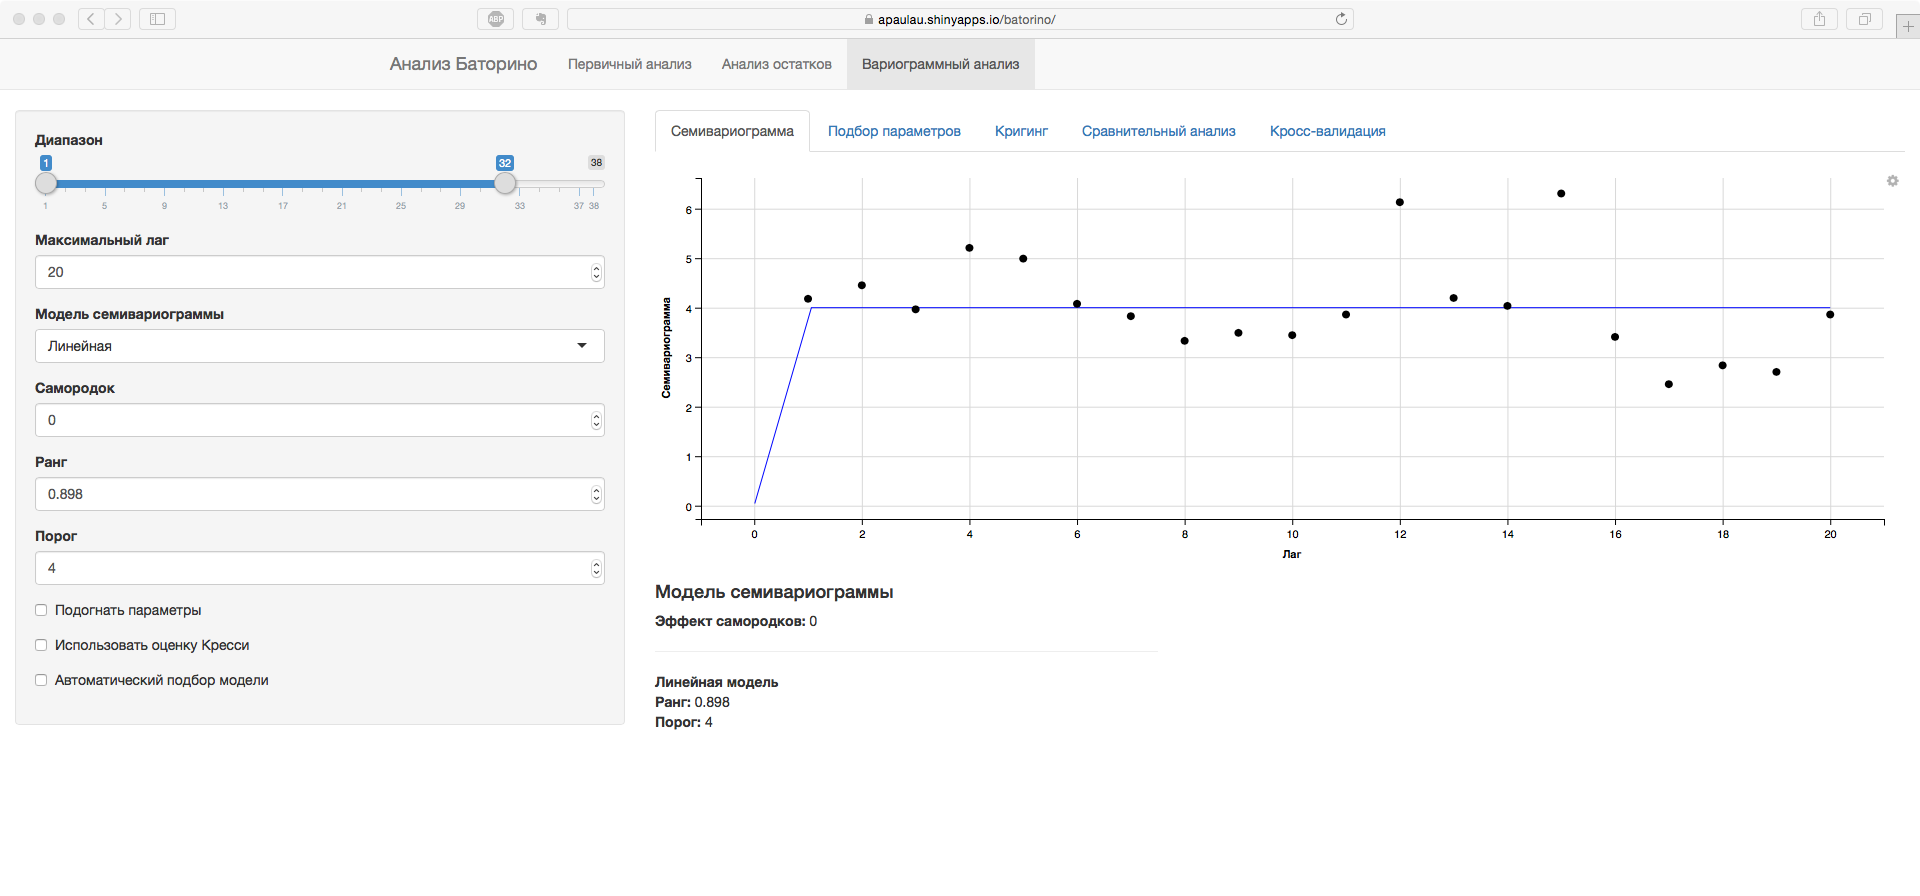
\includegraphics[width=0.9\textwidth]{../../figures/static/4_variogram.png}
  \end{center}
\end{frame}

\begin{frame}
  \frametitle{Модуль вариограммного анализа}
  \framesubtitle{Подбор параметров модели вариограммы}
  \begin{center}
    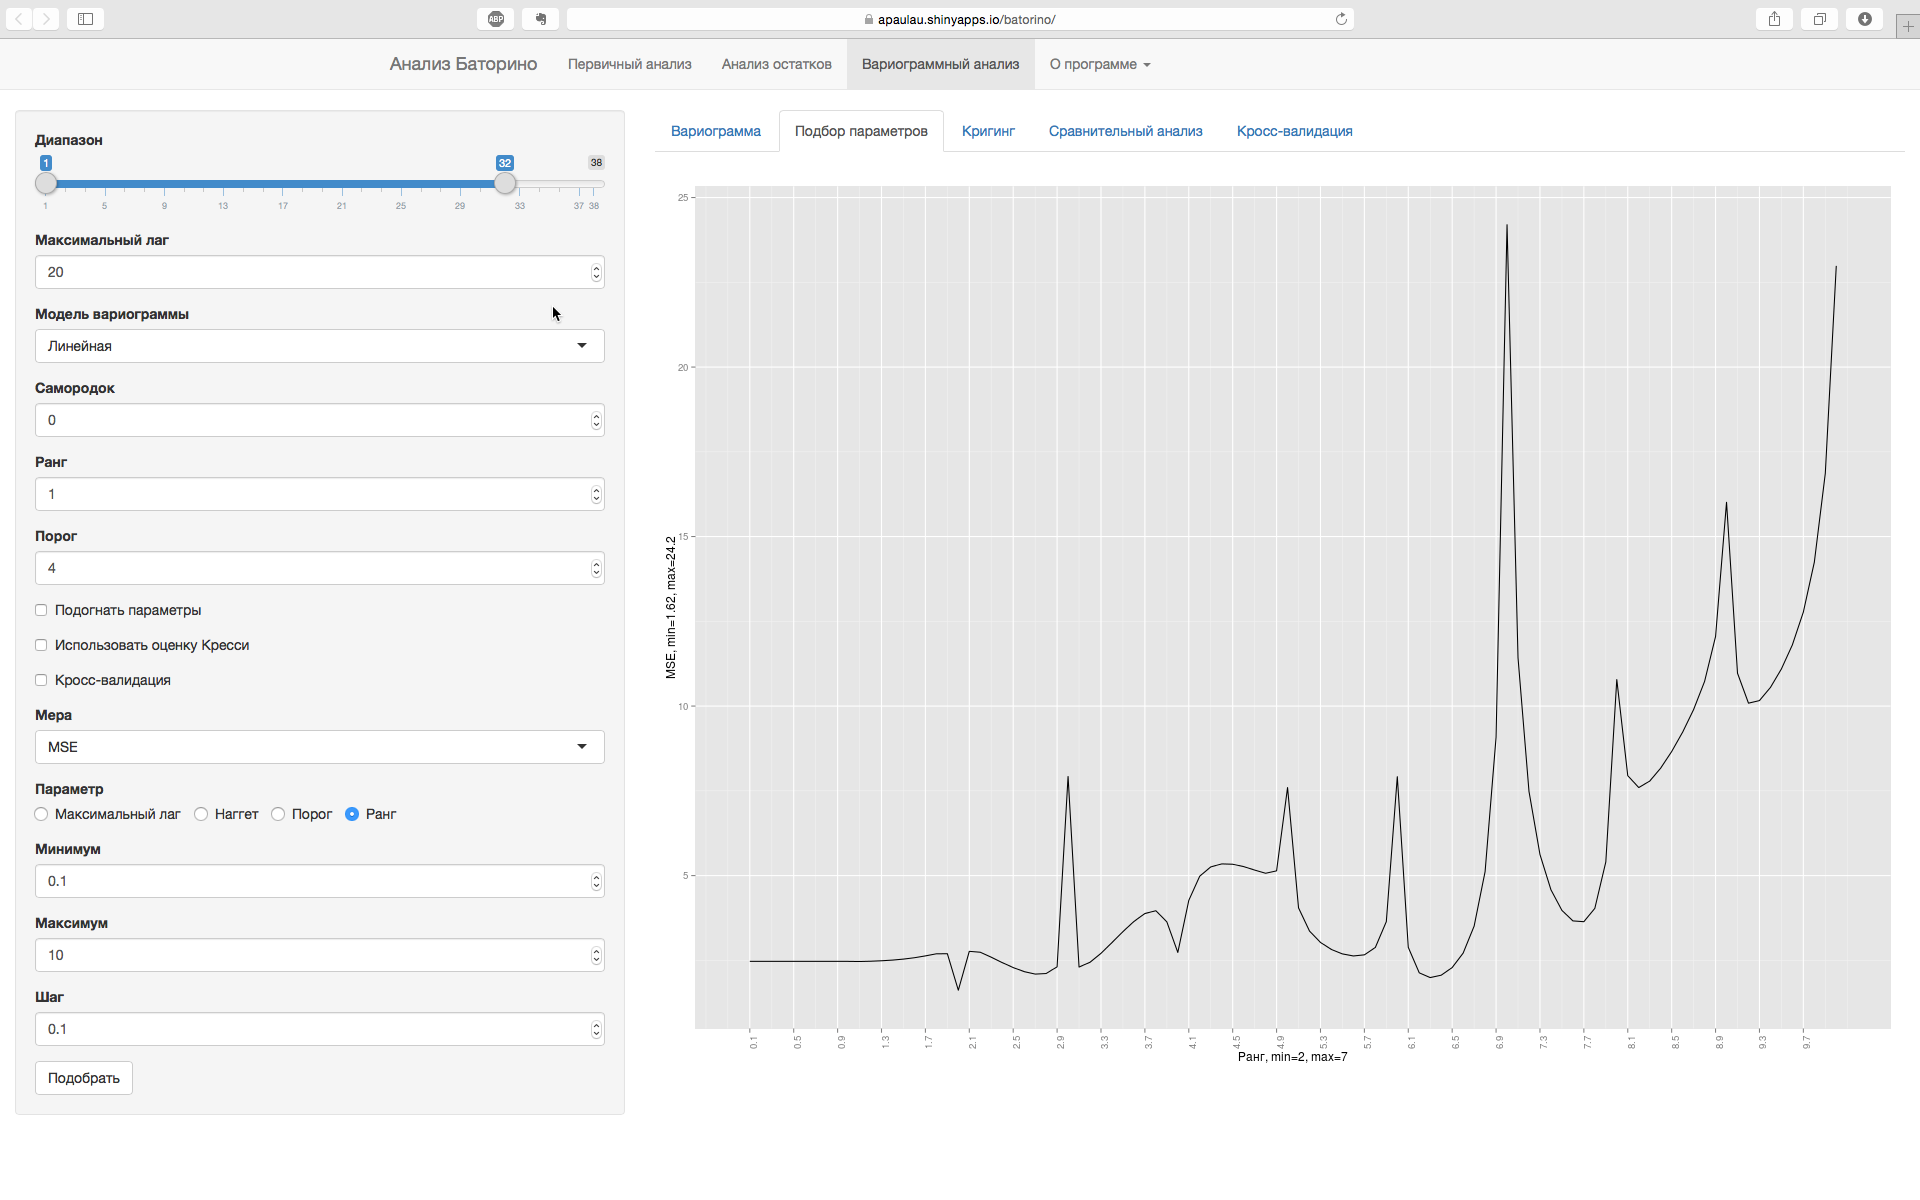
\includegraphics[width=0.9\textwidth]{../../figures/static/5_fit.png}
  \end{center}
\end{frame}

\begin{frame}
  \frametitle{Модуль вариограммного анализа}
  \framesubtitle{Сравнение прогнозных значений}
  \begin{center}
    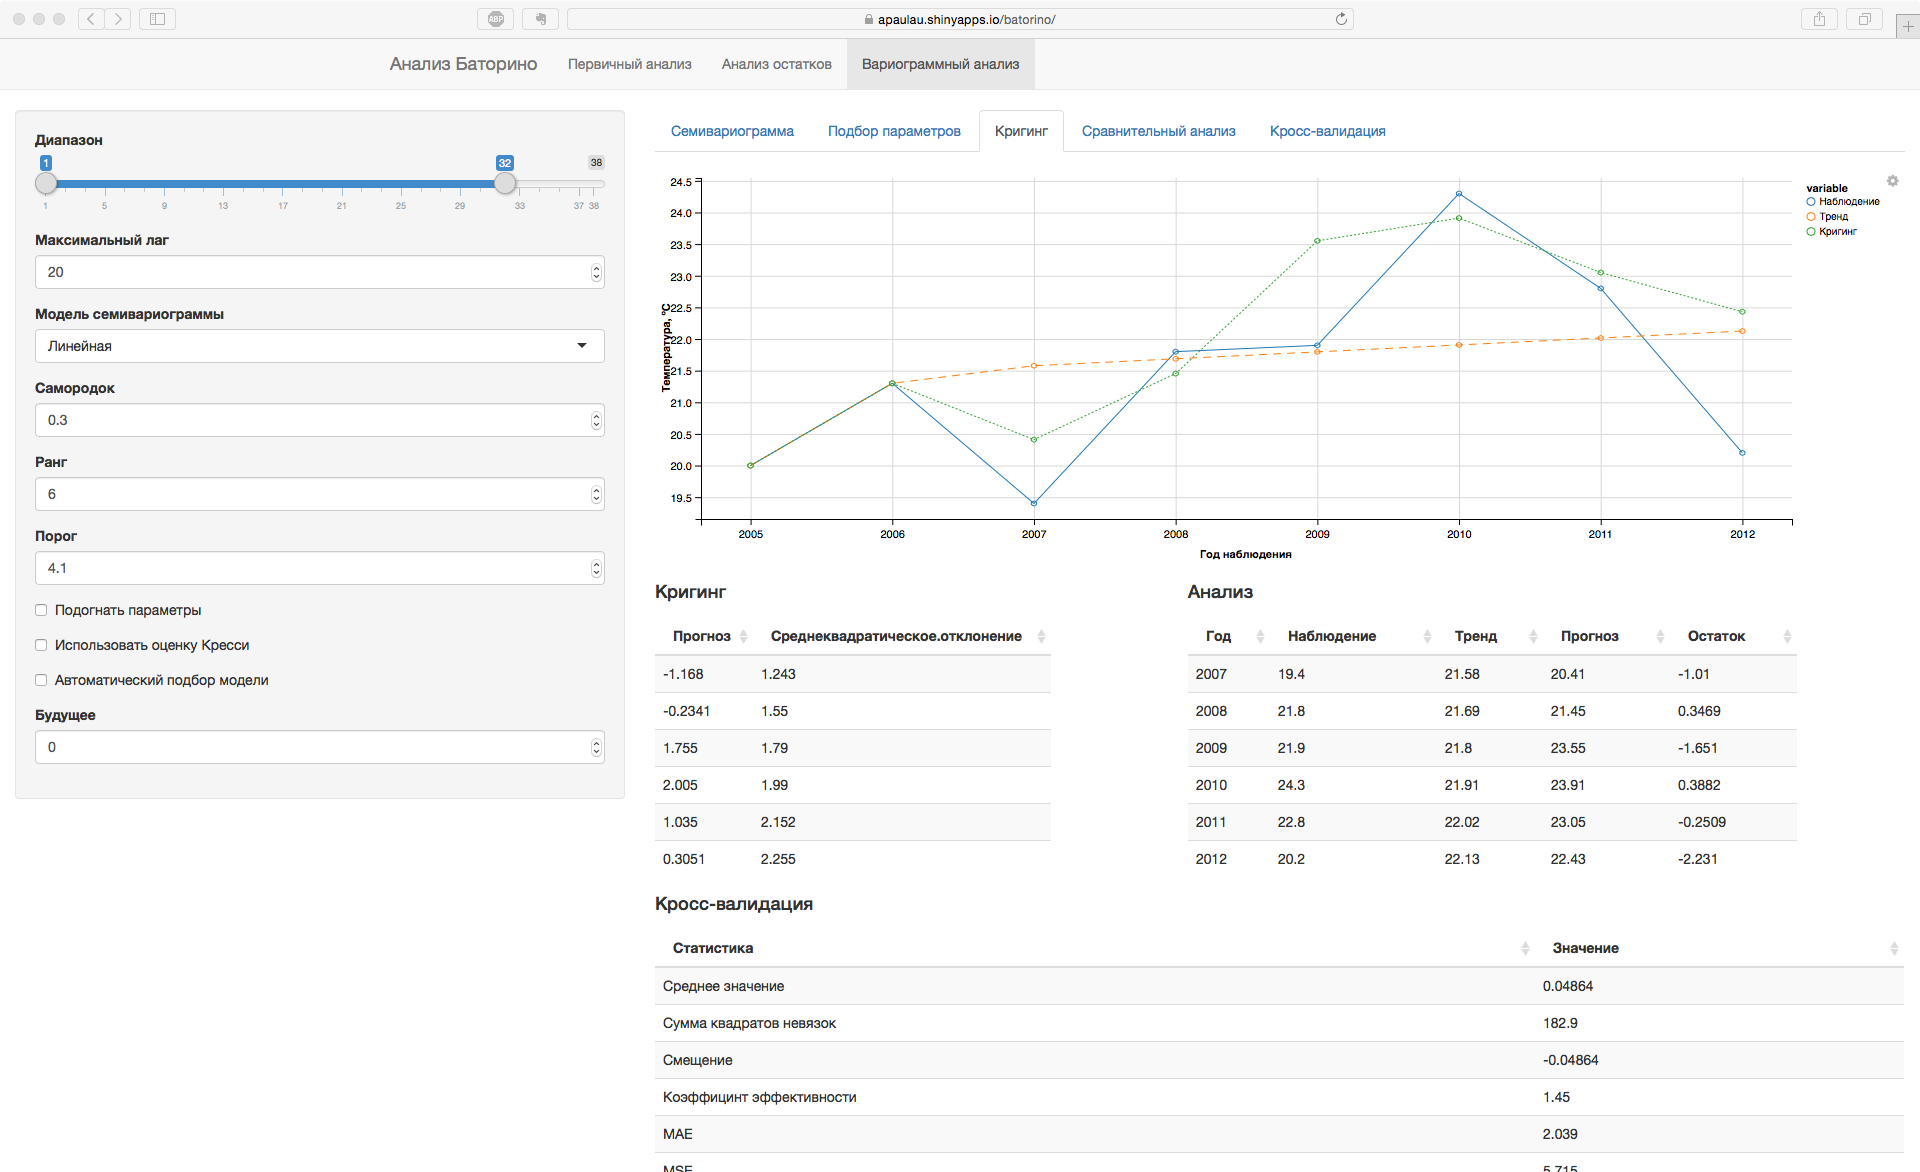
\includegraphics[width=0.9\textwidth]{../../figures/static/6_krige.png}
  \end{center}
\end{frame}

\section{Детерминированный подход}
\begin{frame}
  \frametitle{Детерминированный подход}
  \framesubtitle{Исходные данные}
  \begin{multicols}{2}
    Данные получены от учебно-научного центра <<Нарочанская биологическая станция им. Г.Г.Винберга>>.
    
    \columnbreak
    
    \begin{figure}[h]
      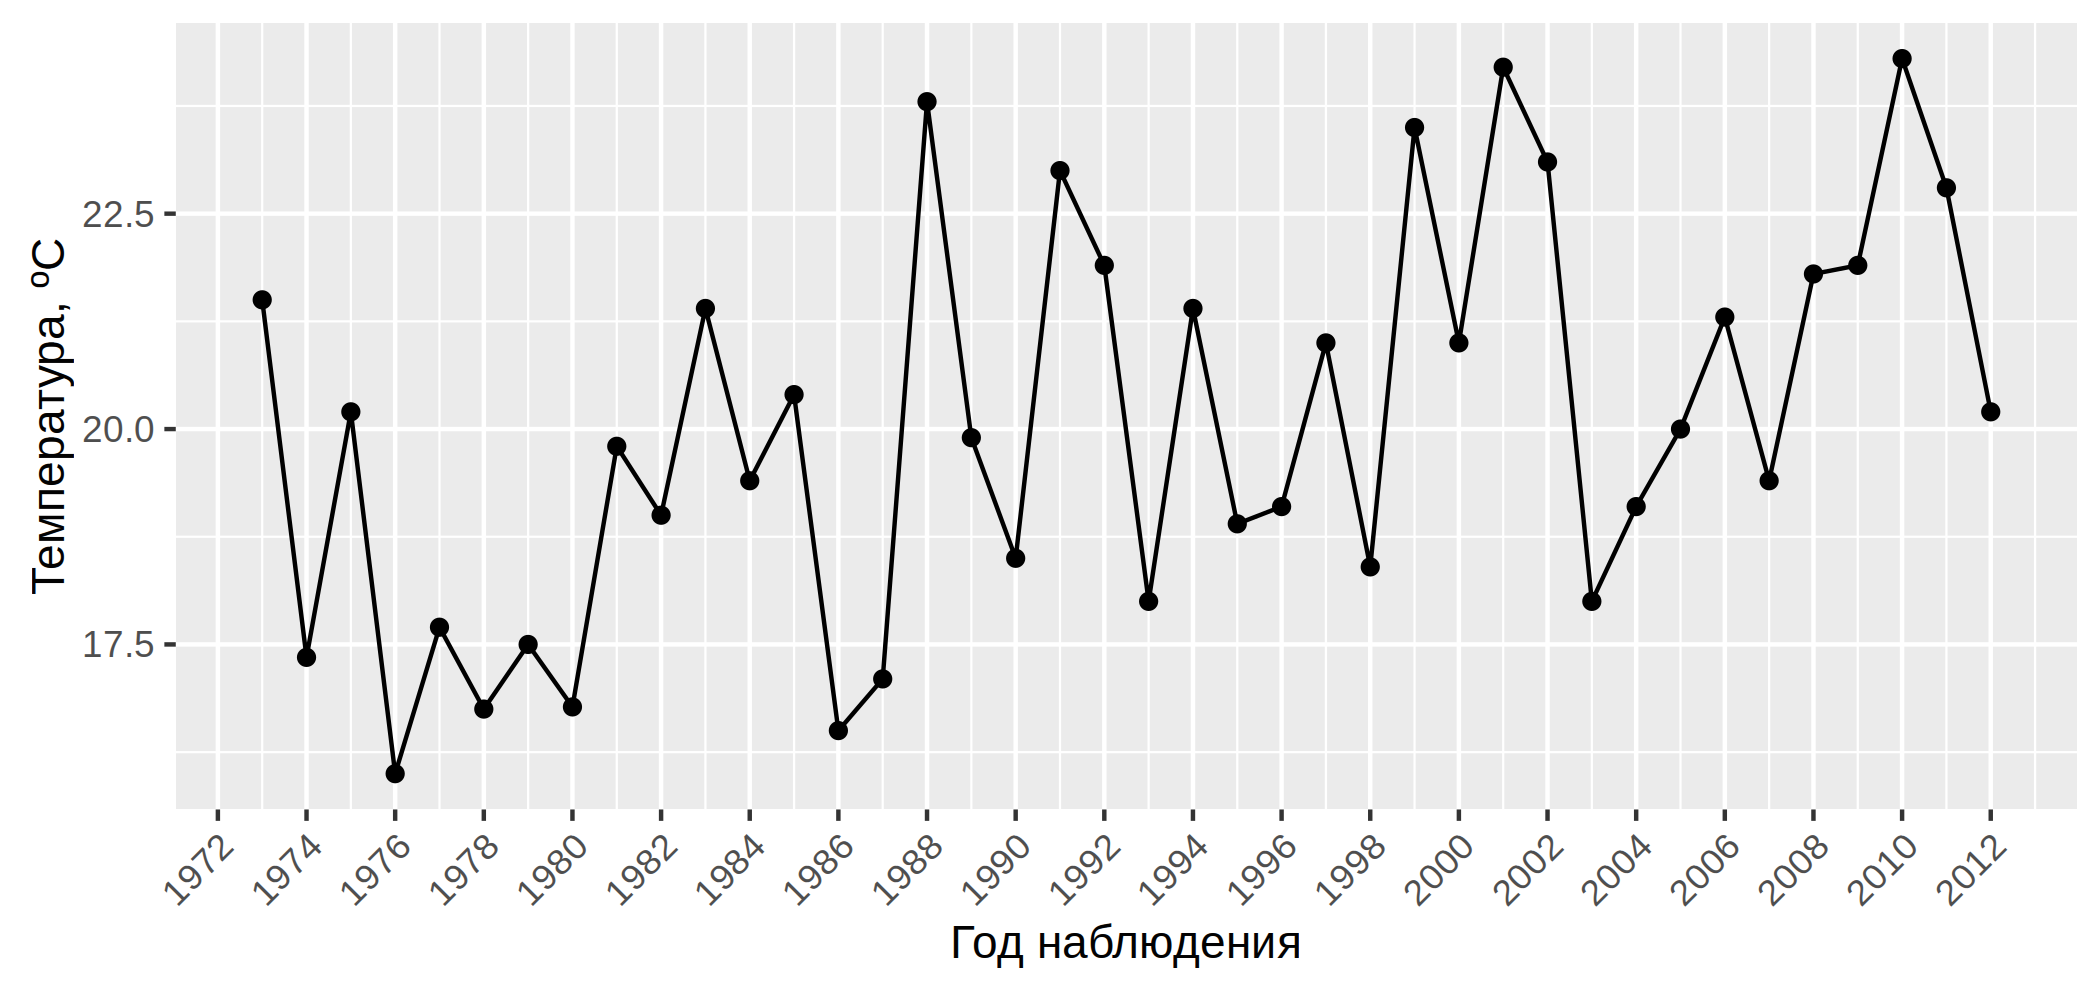
\includegraphics[width=\columnwidth]{../../figures/source.png}
      \caption{Исходные данные}
    \end{figure}
  \end{multicols}
  Исходные данные: выборка $ X(t) $, $ t = \overline{1,n} $, $ n = 38 $, $ X(t) $ --- значение средней температуры воды оз. Баторино в июле месяце для каждого года в период с 1975 по 2012 годы.
\end{frame}

\subsection{Проверка на нормальность}
\begin{frame}
  \frametitle{Детерминированный подход}
  \framesubtitle{Проверка на нормальность}
  \begin{multicols}{2}
  \begin{itemize}
    \item Коэффициент асимметрии $ \descriptive{original}{skew} $ $ \Leftrightarrow $ распределение скошено вправо;
    \item Коэффициент эксцесса $ \descriptive{original}{kurtosis} $ $ \Leftrightarrow $ пик кривой распределения пологий относительного нормального.
  \end{itemize}
  
  \columnbreak
  \begin{figure}[h]
    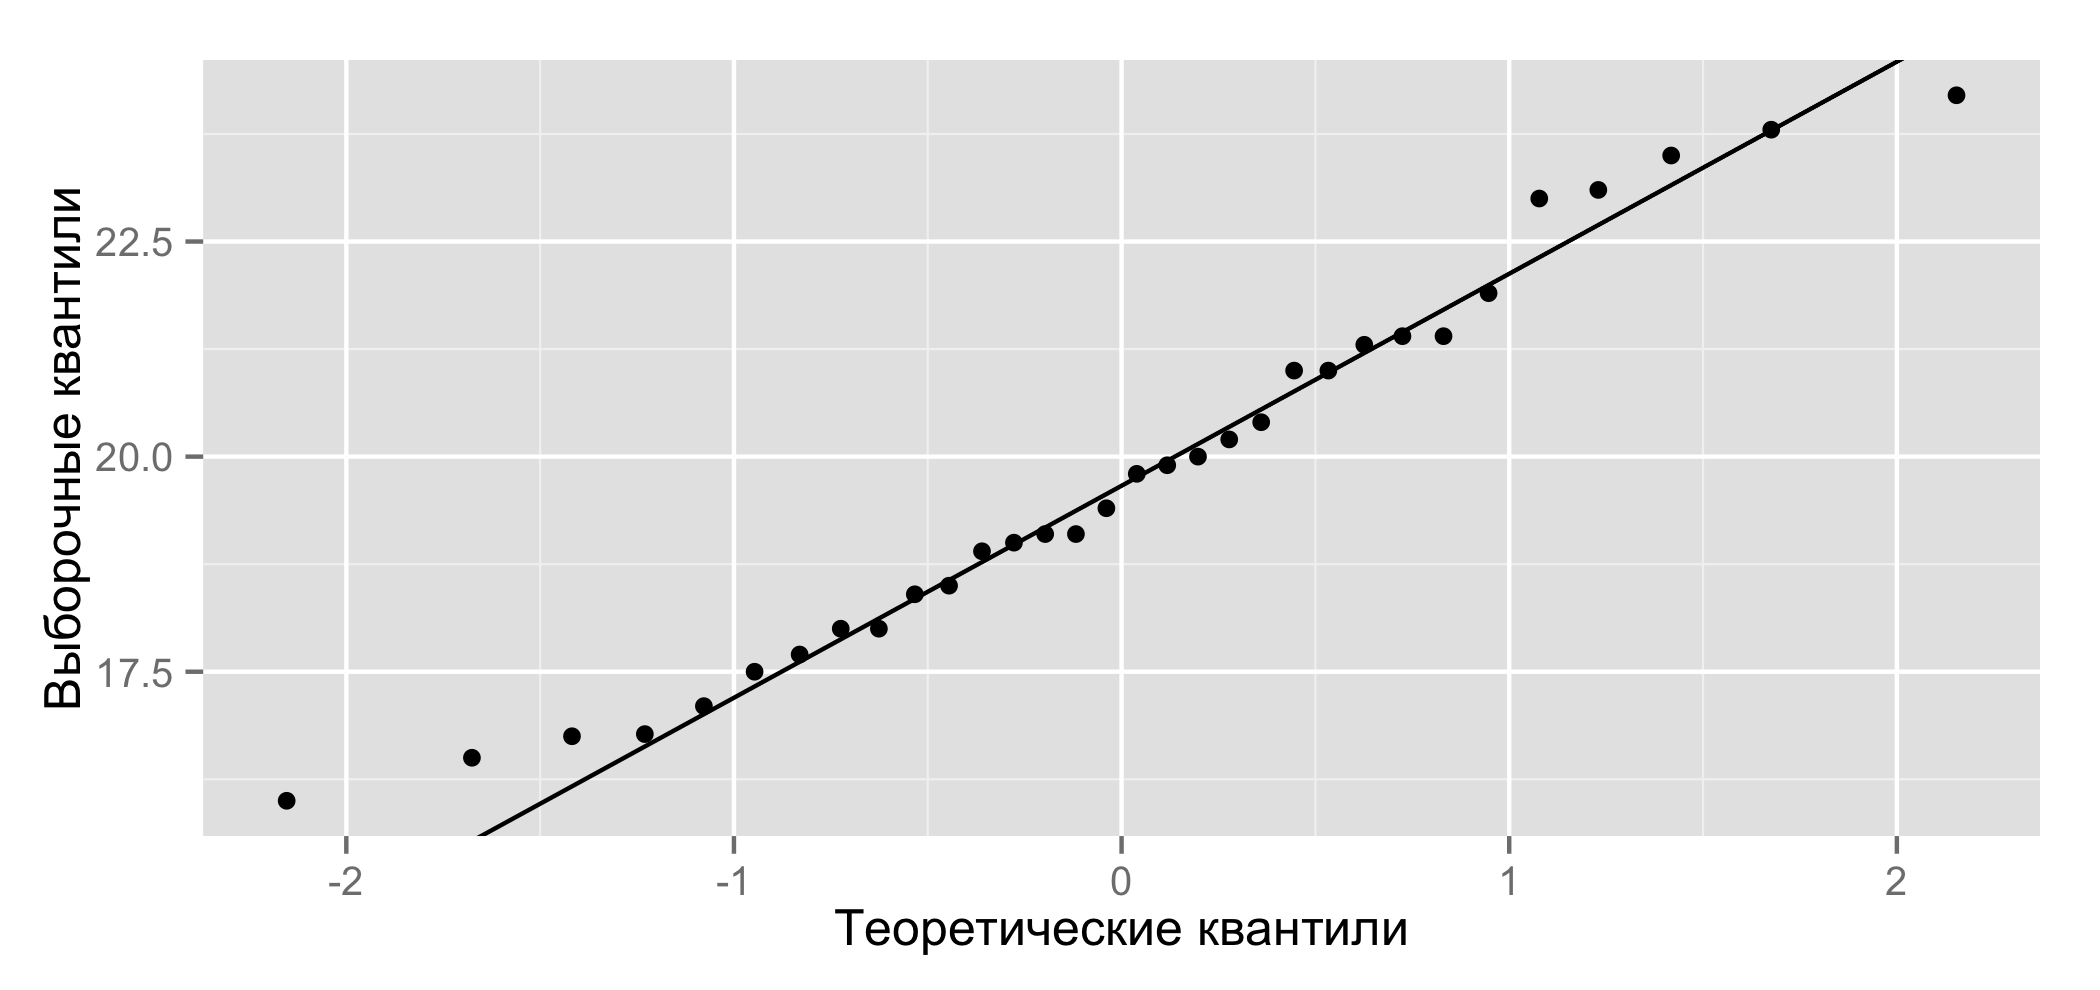
\includegraphics[width=1\linewidth]{../../figures/original/quantile.png}
    \caption{График квантилей}
  \end{figure}
  \end{multicols}
  
  Выборочное распределение близко к нормальному \normaldistr (визуально, критерии Шапиро-Уилка, $\chi^2$-Пирсона и Колмогорова-Смирнова).
\end{frame}

\subsection{Корреляционный анализ}
\begin{frame}
  \frametitle{Детерминированный подход}
  \framesubtitle{Корреляционный анализ}
  \begin{multicols}{2}
  \begin{itemize}
    \item Выбросы в исходных данных отсутствуют (критерий Граббса);
    \item Выборочный коэффициент корреляции $ r_{xt} = \characteristic{original}{correlation} $ --- при уровне значимости $ \alpha=0.05 $ является значимым.
  \end{itemize}
  
  \columnbreak
    \begin{figure}[h]
    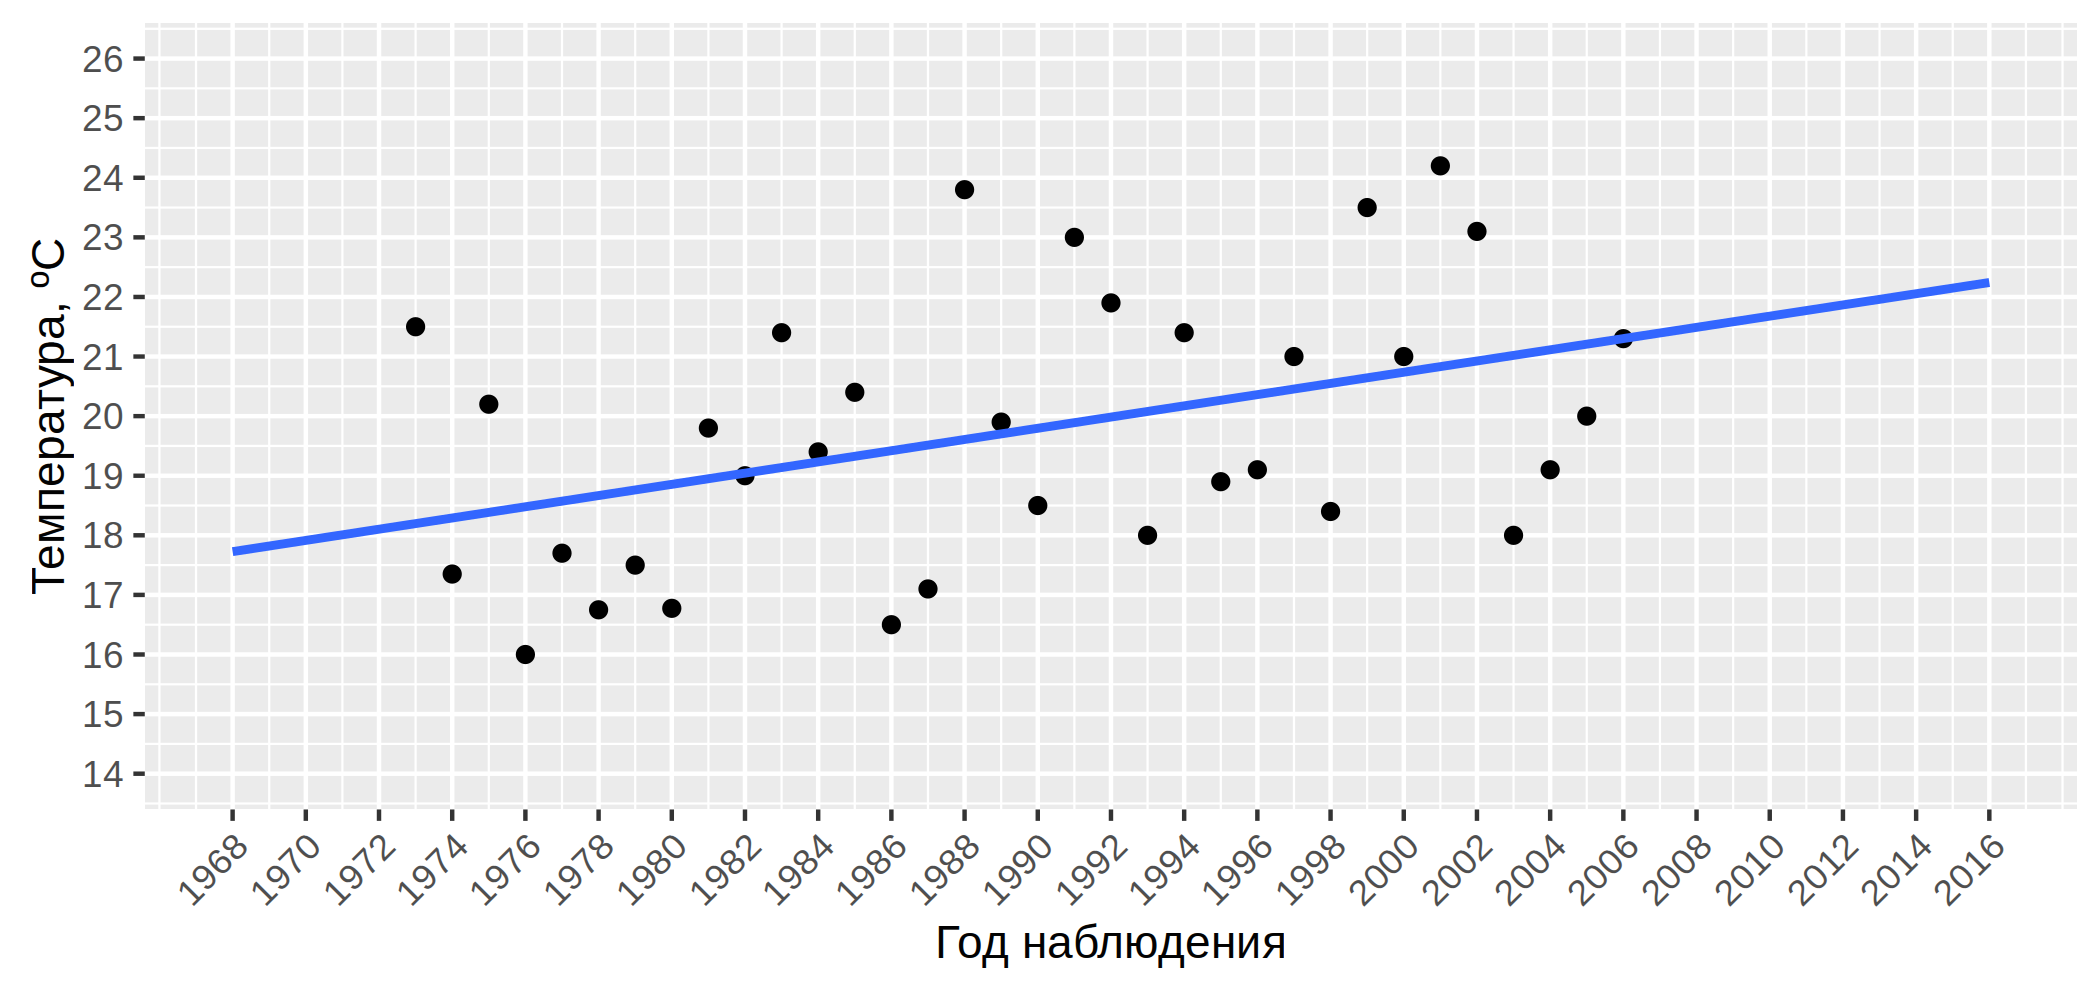
\includegraphics[width=1\linewidth]{../../figures/original/scatterplot.png}
    \caption{Диаграмма рассеяния}
  \end{figure}
  \end{multicols}
\end{frame}

\subsection{Регрессионный анализ}
\begin{frame}
  \frametitle{Детерминированный подход}
  \framesubtitle{Регрессионный анализ: регрессионная модель}
  \begin{multicols}{2}
  Исследуемый временной ряд является аддитивным,
  \begin{equation}
    X(t) = y(t) + \varepsilon(t);
  \end{equation}
  $ y(t) $ --- тренд, $ \varepsilon(t) $ --- нерегулярная составляющая.
  
  \medskip
  
  Найденная модель тренда: $ y(t) = at + b = 0.1014t + 18.0521 $.
  
  \columnbreak
    \begin{figure}[h]
    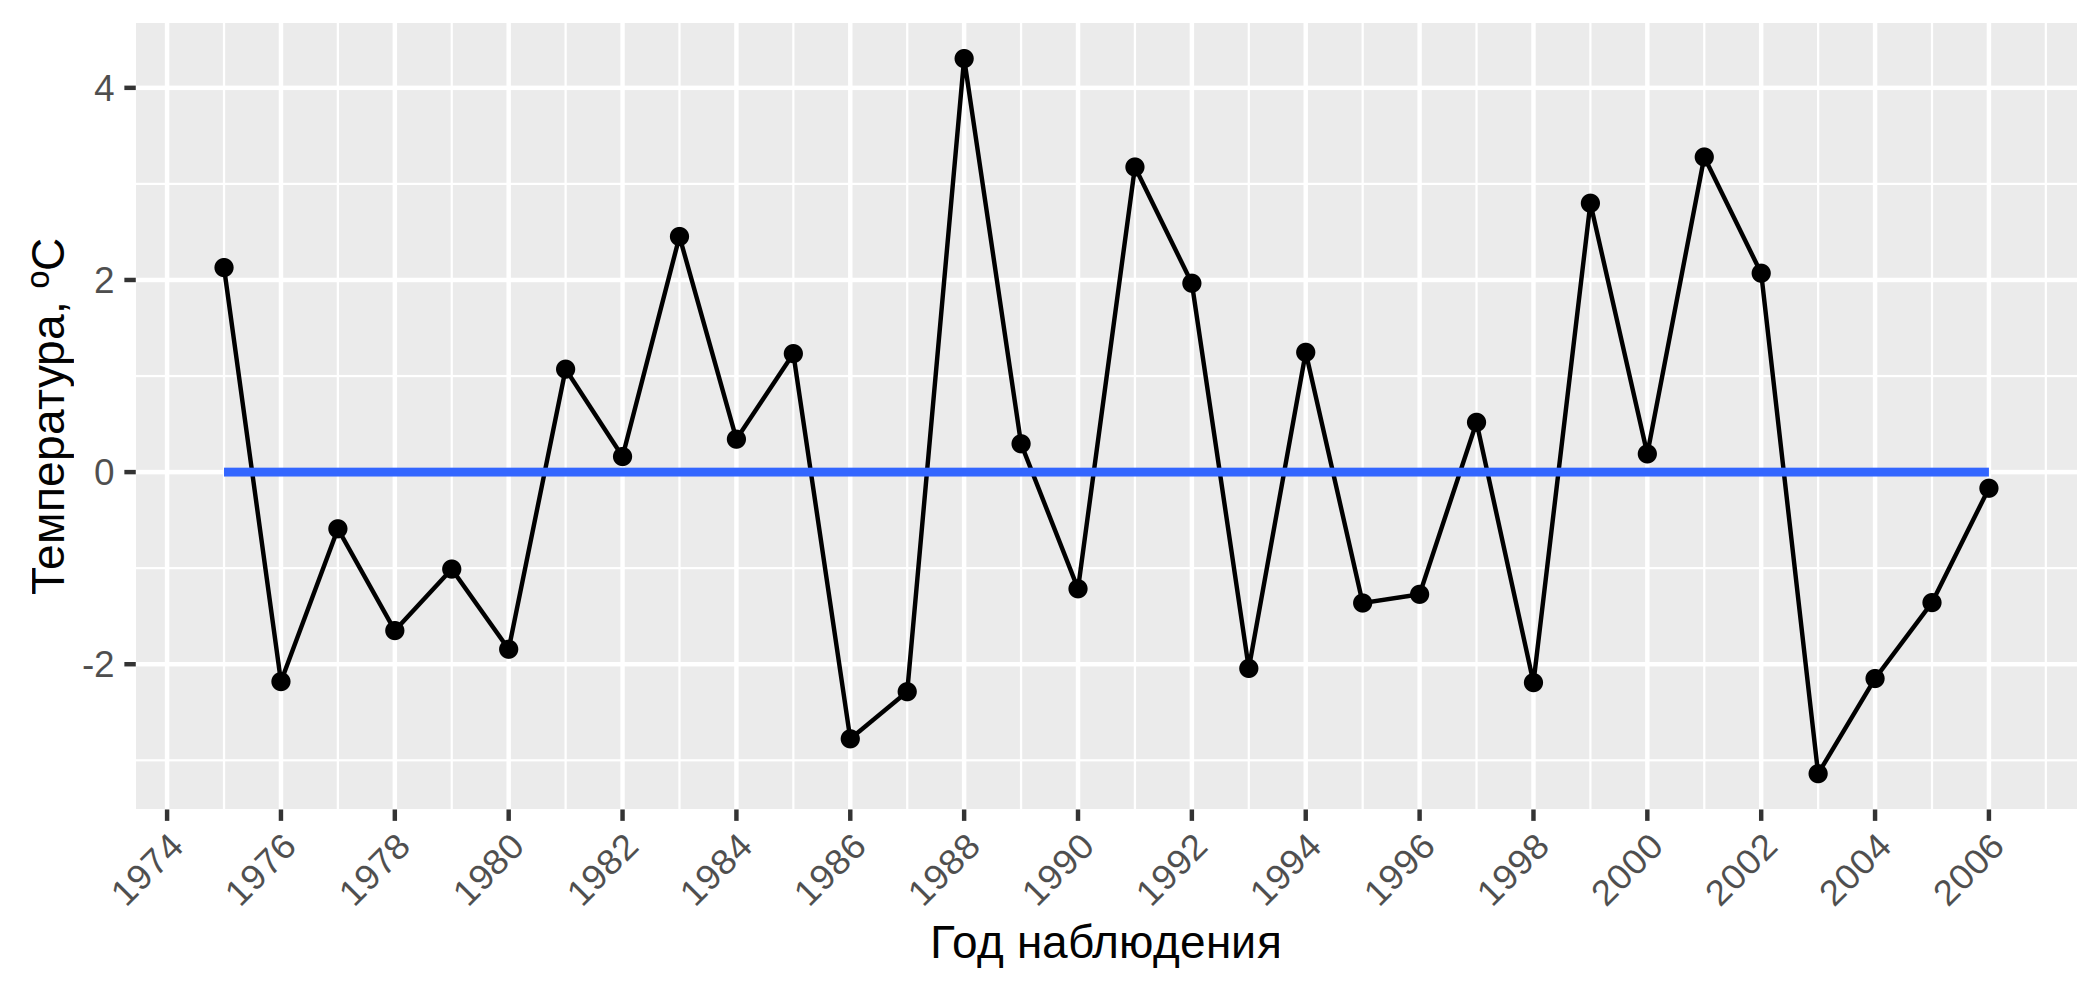
\includegraphics[width=1\linewidth]{../../figures/residual/time-series.png}
    \caption{Ряд остатков $ \varepsilon(t) $}
  \end{figure}
  \end{multicols}
\end{frame}

\begin{frame}
  \frametitle{Детерминированный подход}
  \framesubtitle{Регрессионный анализ: качество регрессионной модели}
  
  % latex table generated in R 3.1.3 by xtable 1.7-4 package
% Thu May 21 14:09:02 2015
\begin{table}[ht]
\centering
\begin{tabular}{rrrr}
  \hline
 & Год & Актуальное & Прогнозное \\ 
  \hline
1 & 2007 & 19.40 & 18.07 \\ 
  2 & 2008 & 21.80 & 18.18 \\ 
  3 & 2009 & 21.90 & 18.29 \\ 
  4 & 2010 & 24.30 & 18.40 \\ 
  5 & 2011 & 22.80 & 18.51 \\ 
  6 & 2012 & 20.20 & 18.62 \\ 
   \hline
\end{tabular}
\caption{Сравнение прогнозных значений (тренда)} 
\label{table:prediction_trend}
\end{table}

  
  \begin{itemize}
    \item Коэффициенты регрессионной модели значимы (критерий Стьюдента, $ \alpha=0.05 $);
    \item Модель адекватна (F-критерий Фишера, $ \alpha = 0.05 $);
    \item Точность модели невысока (поскольку коэффициент детерминации $ \eta^2_{x(t)} = 0.275 $).
  \end{itemize}
\end{frame}

\subsection{Анализ остатков}
\begin{frame}
  \frametitle{Детерминированный подход}
  \framesubtitle{Анализ остатков}
  \begin{figure}[h]
    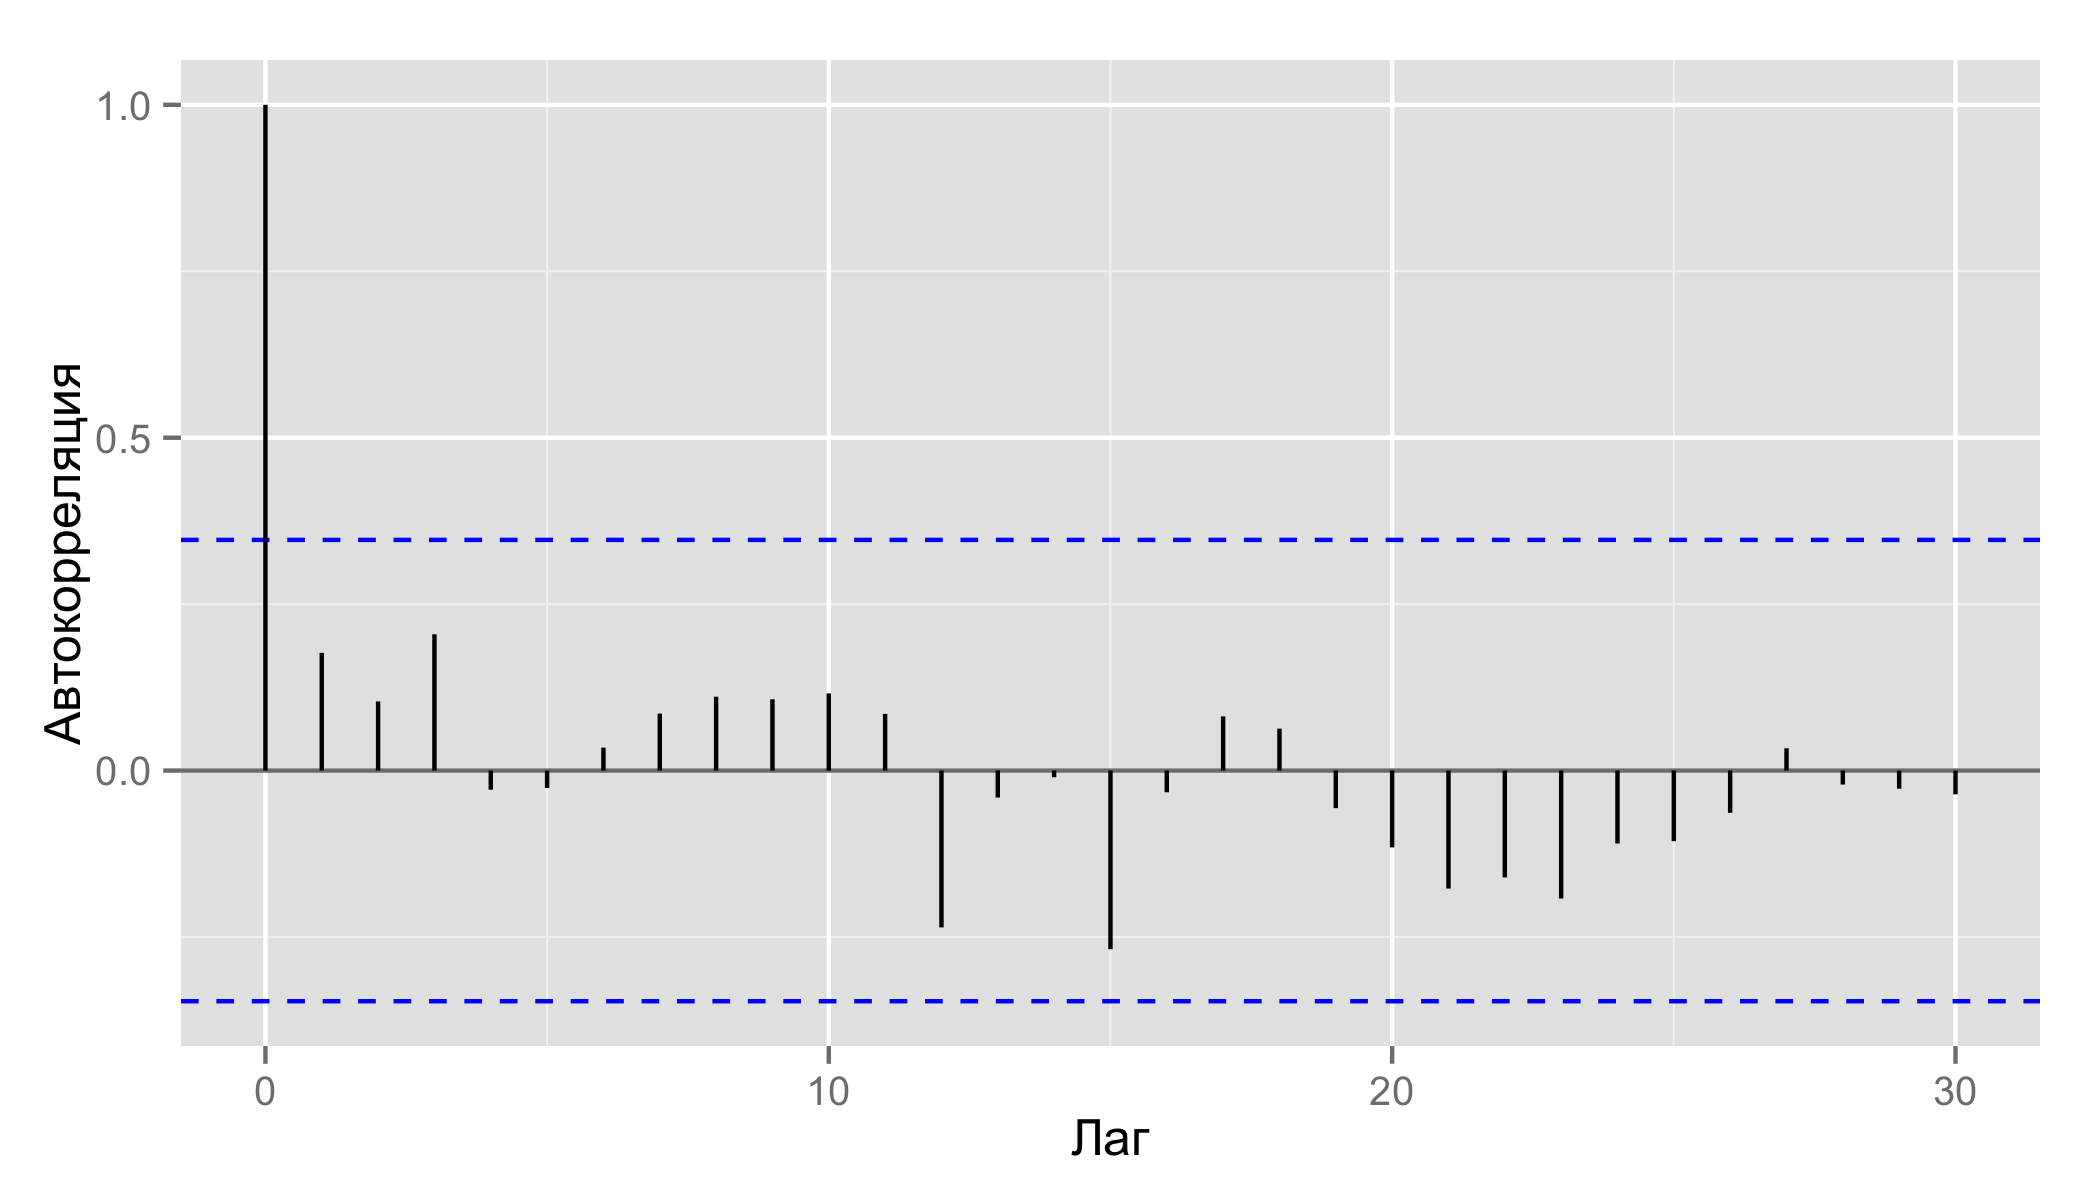
\includegraphics[width=0.7\linewidth]{../../figures/residual/acf.png}
    \caption{Автокорреляционная функция}
  \end{figure}
  
  {\small
  \begin{itemize}
    \item Выборочное распределение близко к \resnormaldistr;
    \item Значимые автокорреляции отсутствуют;
    \item Значения имеют небольшую амплитуду и имеют тенденцию к затуханию $ \Leftrightarrow $ ряд стационарен в широком смысле.
  \end{itemize}
  }
\end{frame}

\section{Геостатистический подход}
\begin{frame}
  \frametitle{Геостатистический подход}
  \framesubtitle{Оценка вариограммы}
  
  Пусть $ X(t),~ t \in \mathbb{Z} $ --- стационарный в широком смысле гауссовский случайный процесс с дискретным временем, нулевым математическим ожиданием и постоянной дисперсией.
  \begin{Definition}
    \textit{Вариограмма} случайного процесса $ X(t), t \in \mathbb{Z} $:
    \begin{equation}
        2 \gamma (h) = V \{ X(t + h) - X(t) \},~ t, h \in \mathbb{Z}.
    \end{equation}

    При этом функция $ \gamma (h), h \in \mathbb{Z} $, называется \textit{семивариограммой}.
  \end{Definition}
  Оценка вариограммы (Матерон):
  \begin{equation}
    \label{eq:matheron}
    2 \tilde{\gamma}(h) = \frac{1}{n - h} \sum_{t = 1}^{n - h}(X(t + h) - X(t))^2, \quad h = \overline{0, n - 1}.
  \end{equation}
\end{frame}

\begin{frame}
  \frametitle{Геостатистический подход}
  \framesubtitle{Первые два момента оценки вариограммы}
\begin{Theorem}
  Для оценки $ 2 \tilde{\gamma}(h) $ имеют место следующие соотношения:
  \begin{equation*}
    E \{2 \tilde{\gamma}(h) \} = 2 \gamma(h), % DIRTY HACK
  \end{equation*}
  \begin{equation*}
    cov(2 \tilde{\gamma}(h_1), 2 \tilde{\gamma}(h_2)) = \frac{2}{(n - h_1)(n - h_2)} \sum_{t = 1}^{n - h_1}\sum_{s = 1}^{n - h_2} (\gamma(t - h_2 - s) +
  \end{equation*}
  \begin{equation*}
    + \gamma(t + h_1 - s) - \gamma(t - s) - \gamma(t + h_1 - s - h_2))^2,
  \end{equation*}
  \begin{equation*}
    V \{ 2 \tilde{\gamma}(h) \} = \frac{2}{(n-h)^2}\sum_{t,s = 1}^{n - h} ( \gamma(t - h - s) + \gamma(t + h - s) - 2\gamma(t - s) )^2,
  \end{equation*}
  где $ \gamma(h) $, --- семивариограмма процесса $ X(t) $, $ h, h_1, h_2 = \overline{0, n - 1} $.
\end{Theorem}
\end{frame}

\begin{frame}
  \frametitle{Геостатистический подход}
  \framesubtitle{Асимптотическое поведение оценки вариограммы}
  \begin{Theorem}
  Если имеет место соотношение $ \sum_{h = -\infty}^{+\infty} \vert \gamma(h) \vert < +\infty $, то
  \begin{equation*}
    \lim_{n \to \infty} (n - \min\{ h_1, h_2 \}) cov\{ 2 \tilde{\gamma}(h_1), 2 \tilde{\gamma}(h_2) \} = 2 \sum_{m = -\infty}^{+\infty} \gamma(m - h_2) +
  \end{equation*}
  \begin{equation*}
    \gamma(m + h_1) - \gamma(m) - \gamma(m + h_1 - h_2))^2,
  \end{equation*}
  \begin{equation*}
    \lim_{n \to \infty} (n - h) V\{ 2 \tilde{\gamma}(h) \} = 2 \sum_{m = -\infty}^{+\infty} \gamma(m - h) + \gamma(m + h) - 2 \gamma(m))^2.
  \end{equation*}
\end{Theorem}
\end{frame}

\begin{frame}
  \frametitle{Геостатистический подход}
  \framesubtitle{Асимптотическое поведение оценки вариограммы}
  \begin{Corollary}
    Из теоремы 2 следует соотношение
    \begin{equation*}
      \lim_{n \to \infty} V\{ 2 \tilde{\gamma}(h) \} = 0, \quad h = \overline{0, n - 1}.
    \end{equation*}
  \end{Corollary}

  \begin{Corollary}
    В силу показанной в теореме 1 несмещённости оценки и вышеприведённого следствия получаем, что оценка вариограммы $ 2\tilde{\gamma}(h) $ является состоятельной в среднеквадратическом смысле для вариограммы $ \gamma(h), h \in \mathbb{Z} $.
  \end{Corollary}
\end{frame}

\subsection{Вариограммный анализ}
\begin{frame}
  \frametitle{Вариограммный анализ}
  \framesubtitle{График экспериментальной вариограммы}
  \begin{multicols}{2}
    Прогнозные значения $ X^{*}(t) $ вычисляются по формуле:
    \begin{equation*}
      X^{*}(t) = y(t) + \varepsilon^{*}(t),
    \end{equation*}
    где $ y(t) $ --- тренд, $ \varepsilon^{*}(t) $ --- значения, вычисленные с помощью кригинга.

  \columnbreak
    \begin{figure}[h]
    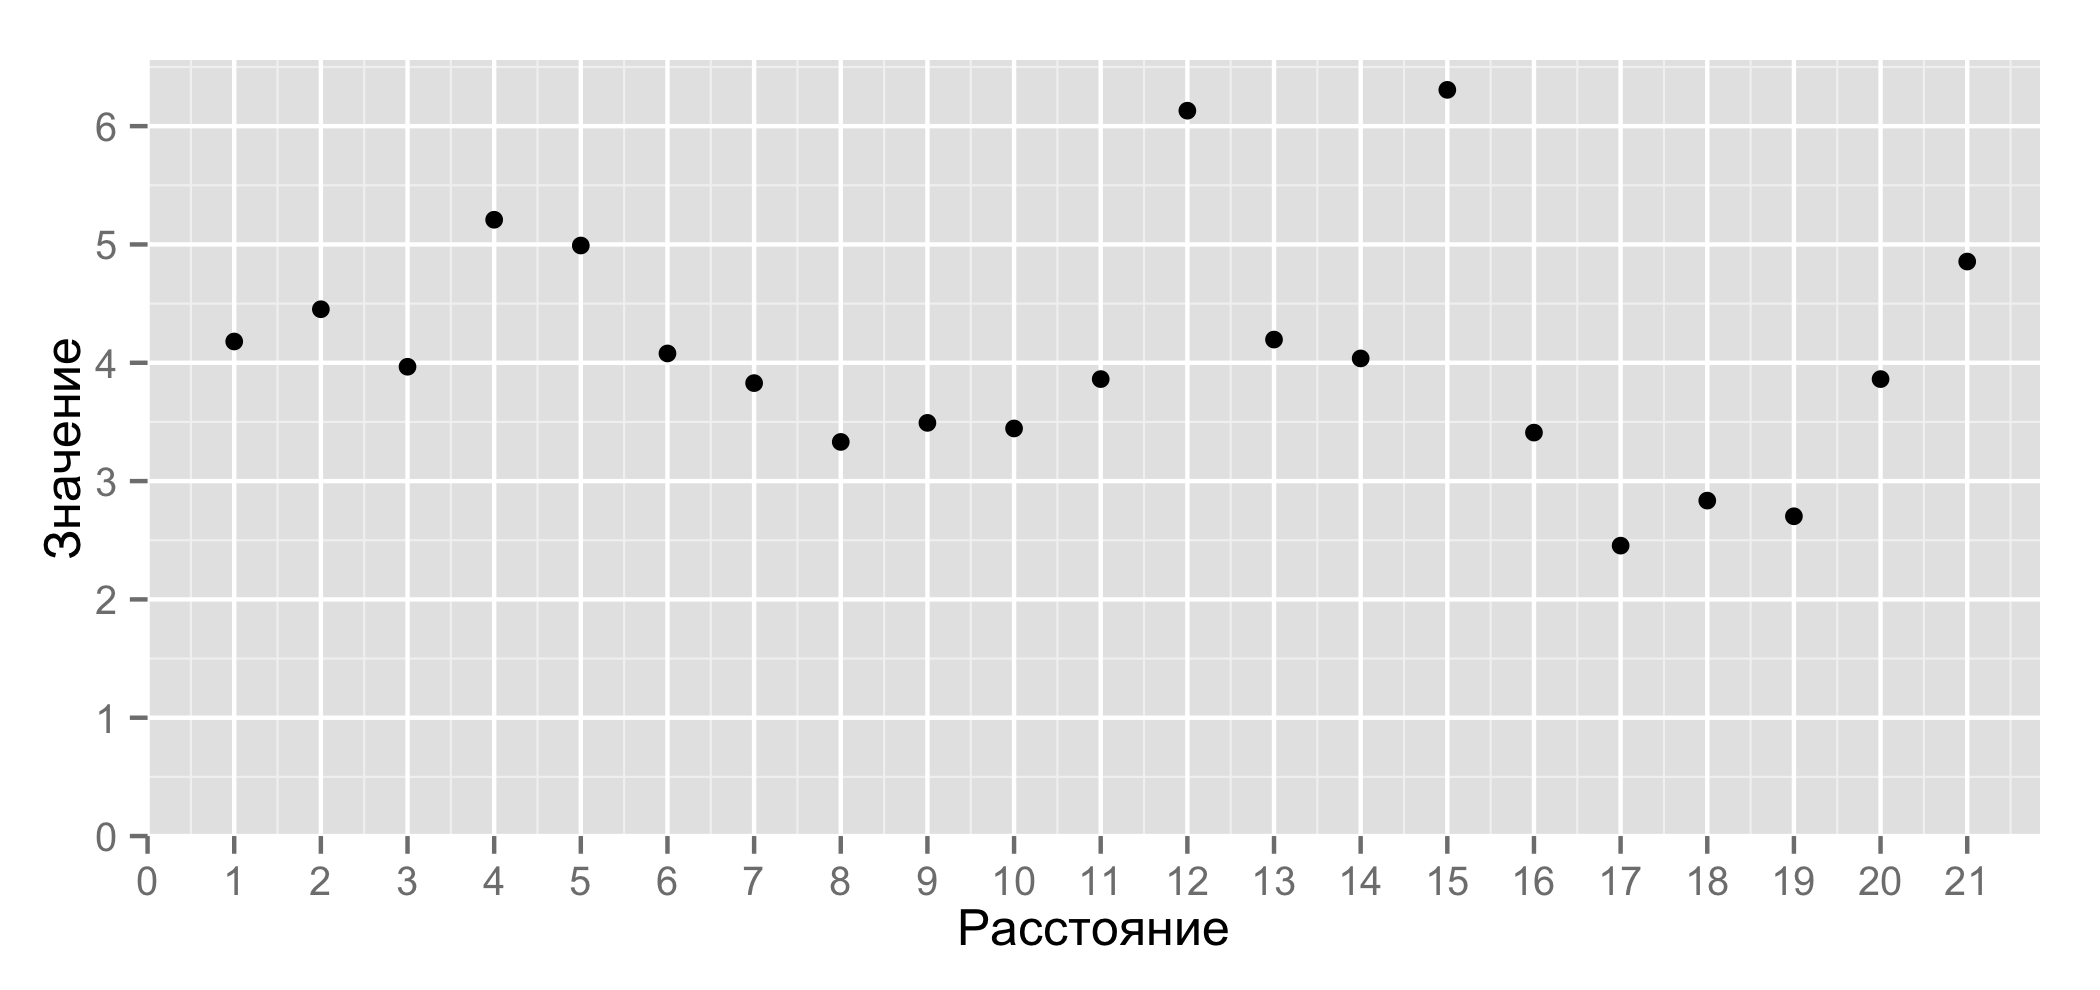
\includegraphics[width=1\linewidth]{../../figures/variogram/lin-variogram.png}
    \caption{Оценка семивариограммы Матерона}
  \end{figure}
  \end{multicols}
    Для оценки качества модели используются
    \begin{itemize}
      \item коэффициент корреляции $ r_{\varepsilon\varepsilon^{*}} $;
      \item Среднеквадратическая ошибка ($ n $ --- объём выборки):
        \begin{equation}
        \label{eq:mse}
          MSE = \frac{1}{n} \sum_{i=1}^{n} (\varepsilon(t_i) - \varepsilon^{*}(t_i))^2.
        \end{equation}
    \end{itemize}
  
\end{frame}

\begin{frame}
  \frametitle{Вариограммный анализ}
  \framesubtitle{Линейная модель}
  \begin{multicols}{2}
    \begin{small}
      Общий вид модели:
      \begin{equation}\begin{gathered}
        \label{eq:lin}
        \widehat{\gamma}(h) = c_0 + Lin(h) = \\ = \left\{
        \begin{array}{l l}
          c_0 + b \cdot h, & h > 0, \\
          c_0, & h \leq 0,
        \end{array} \right.
      \end{gathered}\end{equation}
      где $ b $ -- параметр, отвечающий за угол наклона, $ c_0 $ --- эффект самородков.
      
      \medskip
      
      Подобранная модель:
      \begin{equation}
        \label{eq:gamma1}
        \widehat{\gamma}_1(h) = Lin(h), \quad b = 4
      \end{equation}
      
      Показатели качества
      \begin{equation*}
        r_{\varepsilon\varepsilon^{*}} = -0.09129, \quad MSE = 6.324
      \end{equation*}
    \end{small}
    
    \columnbreak
    \begin{figure}[H]
      \begin{center}
        \begin{minipage}[H]{0.95\linewidth}
          \begin{center}
            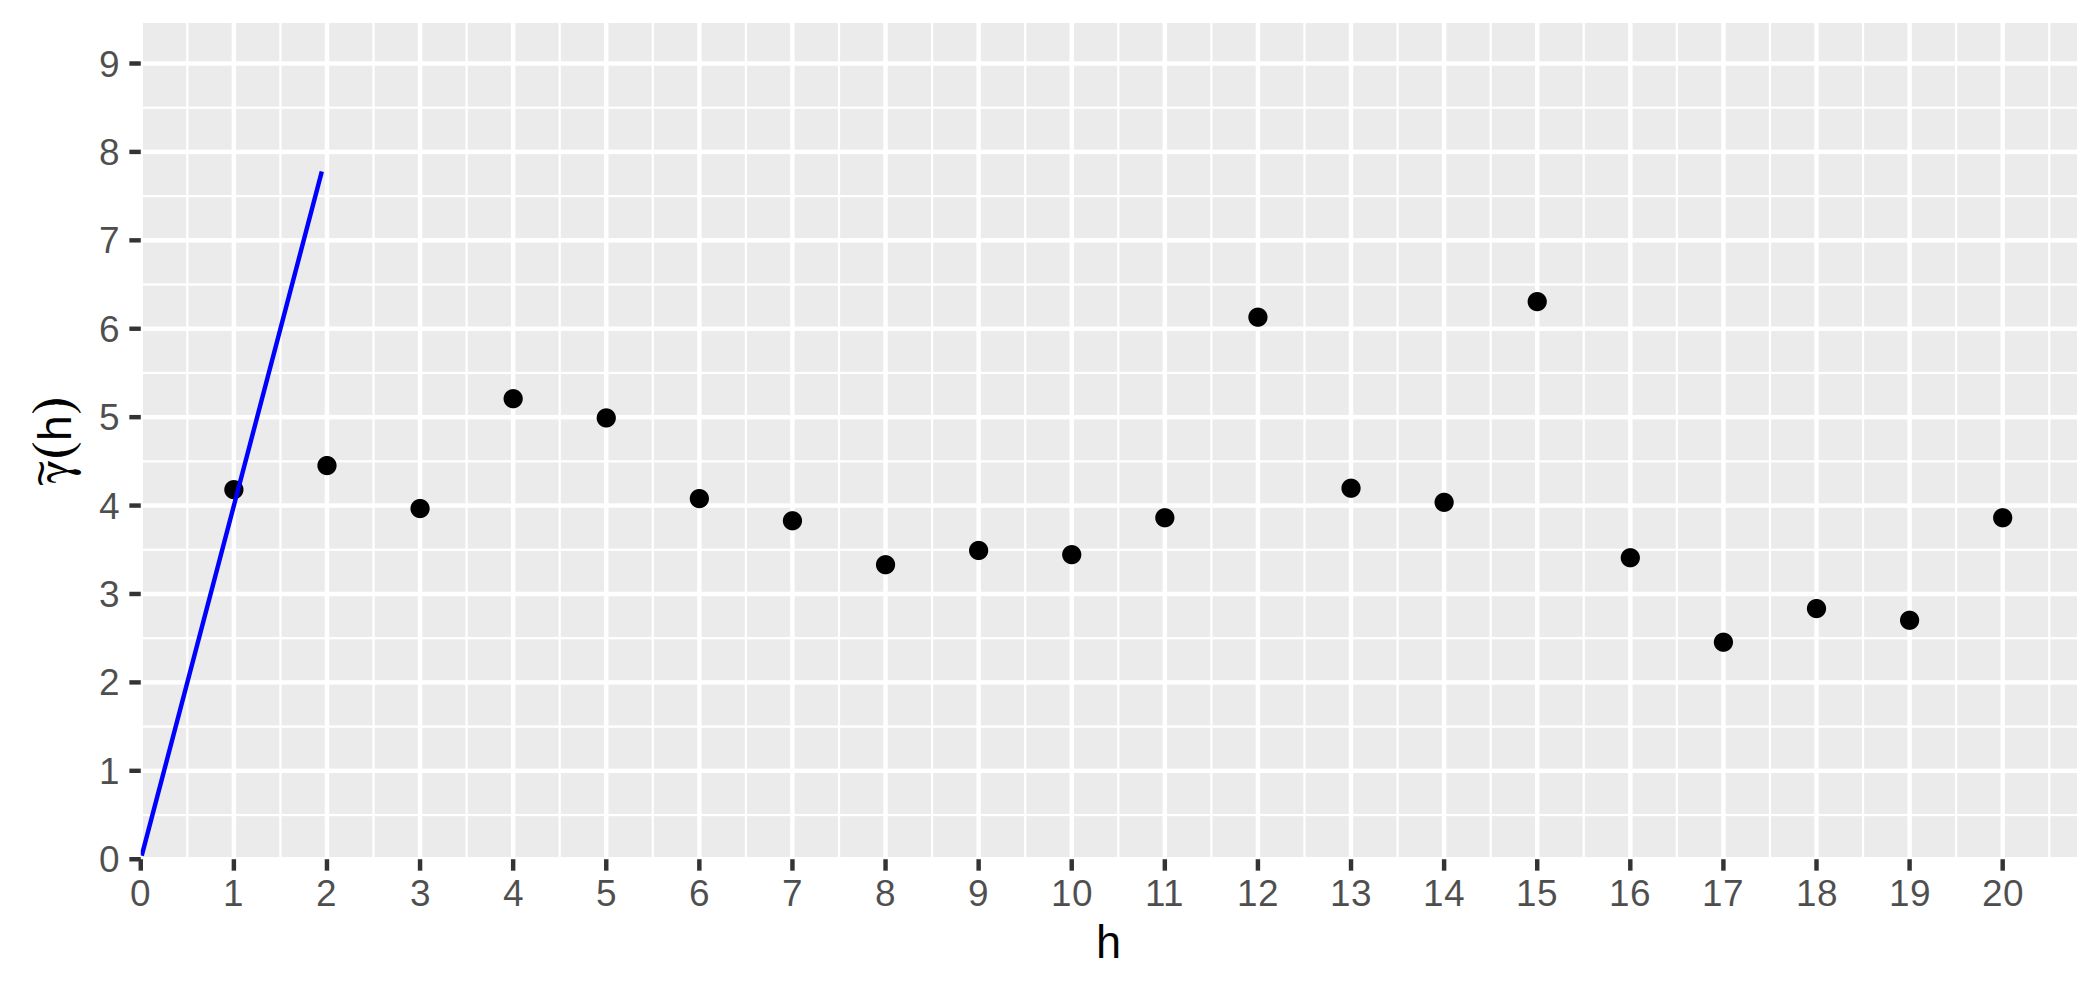
\includegraphics[width=1\linewidth]{../../figures/variogram/lin-modeled.png} \\ Модель семивариограммы $\widehat{\gamma}_1(h)$
          \end{center}
        \end{minipage}
        \\
        \begin{minipage}[H]{0.95\linewidth}
          \begin{center}
            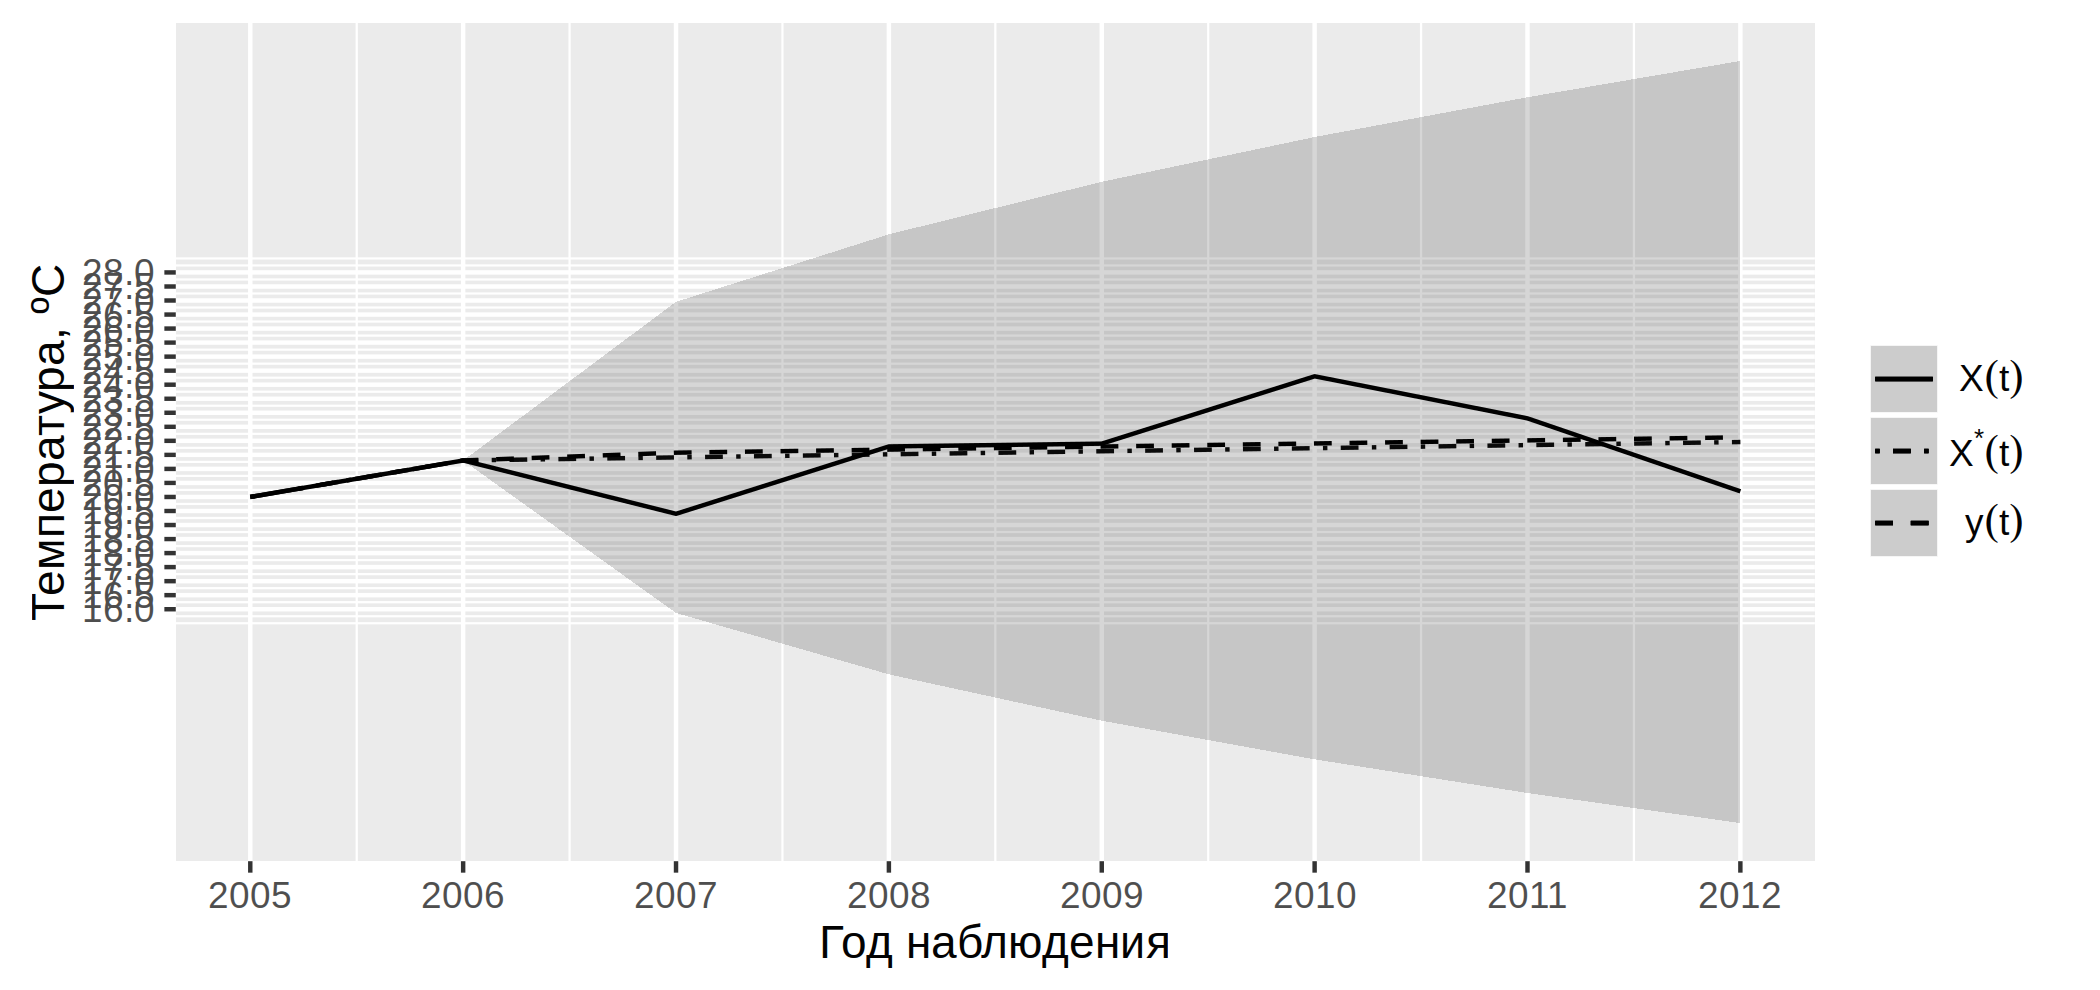
\includegraphics[width=1\linewidth]{../../figures/variogram/lin-cross-prediction.png} \\ Прогноз по модели $\widehat{\gamma}_1(h)$
          \end{center}
        \end{minipage}
      \end{center}
    \end{figure}
  \end{multicols}
\end{frame}

\begin{frame}
  \frametitle{Вариограммный анализ}
  \framesubtitle{Чистый эффект самородков}
  \begin{multicols}{2}
    \begin{small}
      Общий вид модели:
      \begin{equation}\begin{gathered}
        \label{eq:nug}
        \widehat{\gamma}(h) = c \cdot Nug(h) = \\ = \left\{
        \begin{array}{l l}
          0, & h = 0, \\
          c, & h \neq 0,
        \end{array} \right.
      \end{gathered}\end{equation}
      где $ b $ -- параметр, отвечающий за угол наклона, $ c_0 $ --- эффект самородков.
      
      \medskip
      
      Подобранная модель:
      \begin{equation}
        \label{eq:gamma2}
        \widehat{\gamma}_2(h) = 4.04 \cdot Nug(h).
      \end{equation}
      
      Показатели качества
      \begin{equation*}
        r_{\varepsilon\varepsilon^{*}} = -1, \quad MSE = 4.199
      \end{equation*}
    \end{small}
    
    \columnbreak
    \begin{figure}[H]
      \begin{center}
        \begin{minipage}[H]{0.95\linewidth}
          \begin{center}
            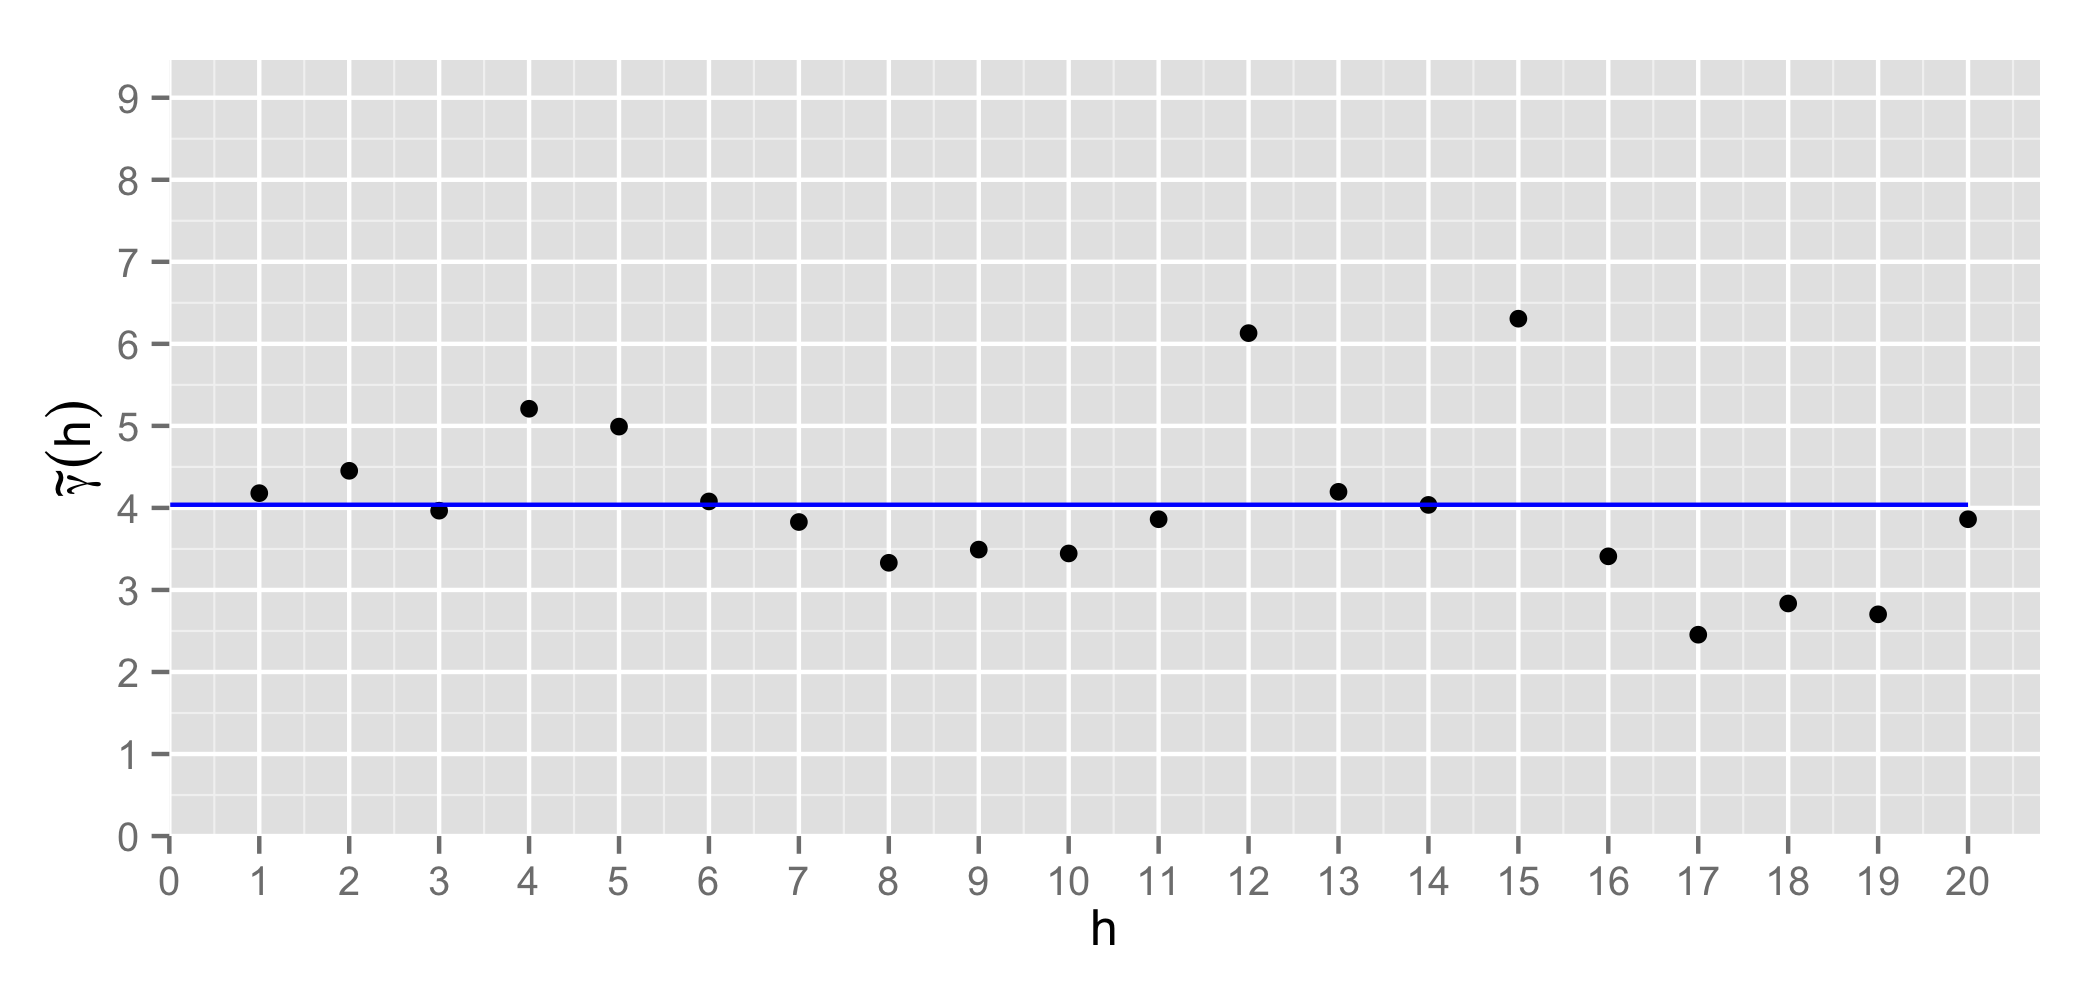
\includegraphics[width=1\linewidth]{../../figures/variogram/lin-fit-modeled.png} \\ Модель семивариограммы $\widehat{\gamma}_2(h)$
          \end{center}
        \end{minipage}
        \\
        \begin{minipage}[H]{0.95\linewidth}
          \begin{center}
            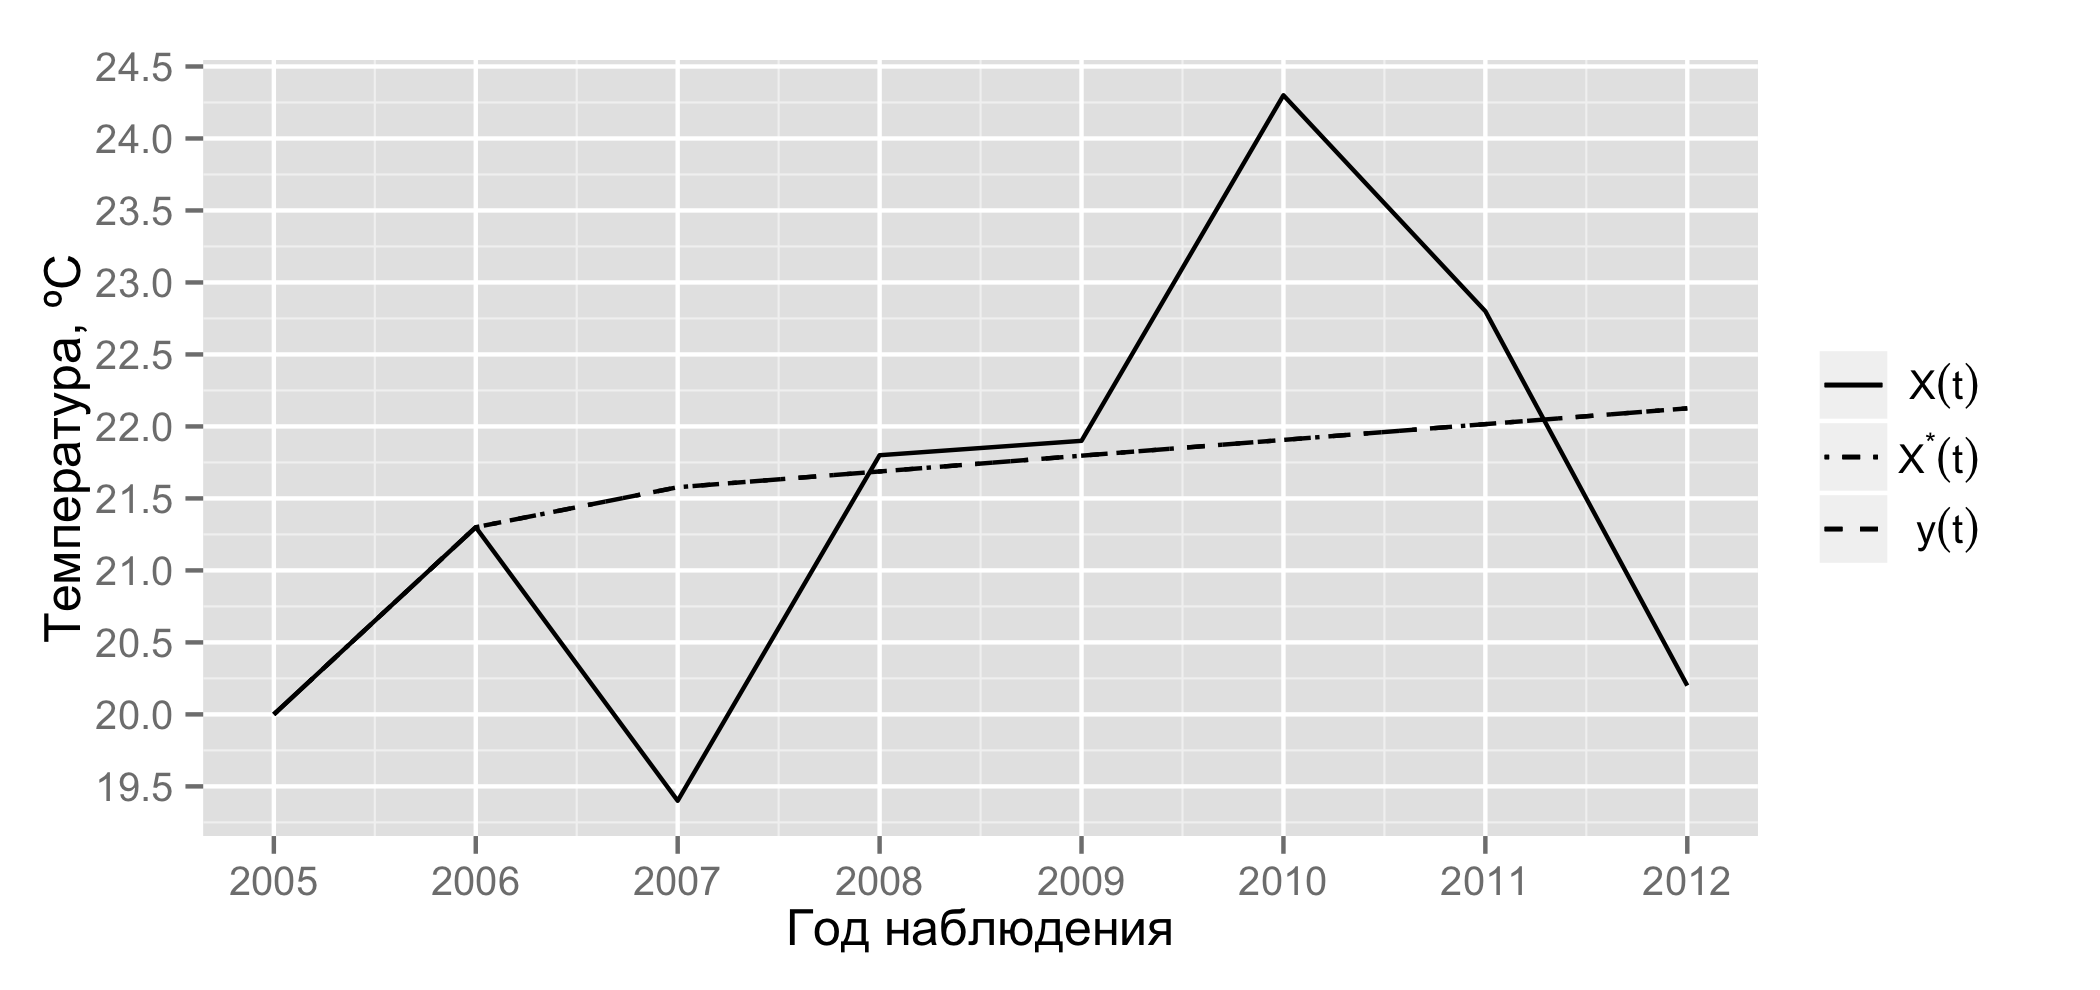
\includegraphics[width=1\linewidth]{../../figures/variogram/lin-fit-cross-prediction.png} \\ Прогноз по модели $\widehat{\gamma}_2(h)$
          \end{center}
        \end{minipage}
      \end{center}
    \end{figure}
  \end{multicols}
\end{frame}

\begin{frame}
  \frametitle{Вариограммный анализ}
  \framesubtitle{Линейная модель с порогом}
  \begin{multicols}{2}
    \begin{small}
      Общий вид модели:
      \begin{equation}\begin{gathered}
      \label{eq:linsill}
        \widehat{\gamma}(h) = c_0 + c \cdot Lin(h, a) = \\
        = \left\{
        \begin{array}{l l}
         c_0 + c \cdot \frac{h}{a}, & 0 \leq h \leq a, \\
         c_0 + c, & h > a,
        \end{array} \right.
      \end{gathered}\end{equation}
      где $ c_0 $ -- эффект самородков, $ c $ -- порог, $ a $ -- ранг.
      
      \medskip
      
      Подобранная модель:
      \begin{equation}
      \label{eq:gamma4}
        \widehat{\gamma}_4(h) = 4 \cdot Lin(h, 2).
      \end{equation}
      
      Показатели качества
      \begin{equation*}
        r_{\varepsilon\varepsilon^{*}} = 0.152, \quad MSE = 18.69
      \end{equation*}
    \end{small}
    
    \columnbreak
    \begin{figure}[H]
      \begin{center}
        \begin{minipage}[H]{0.95\linewidth}
          \begin{center}
            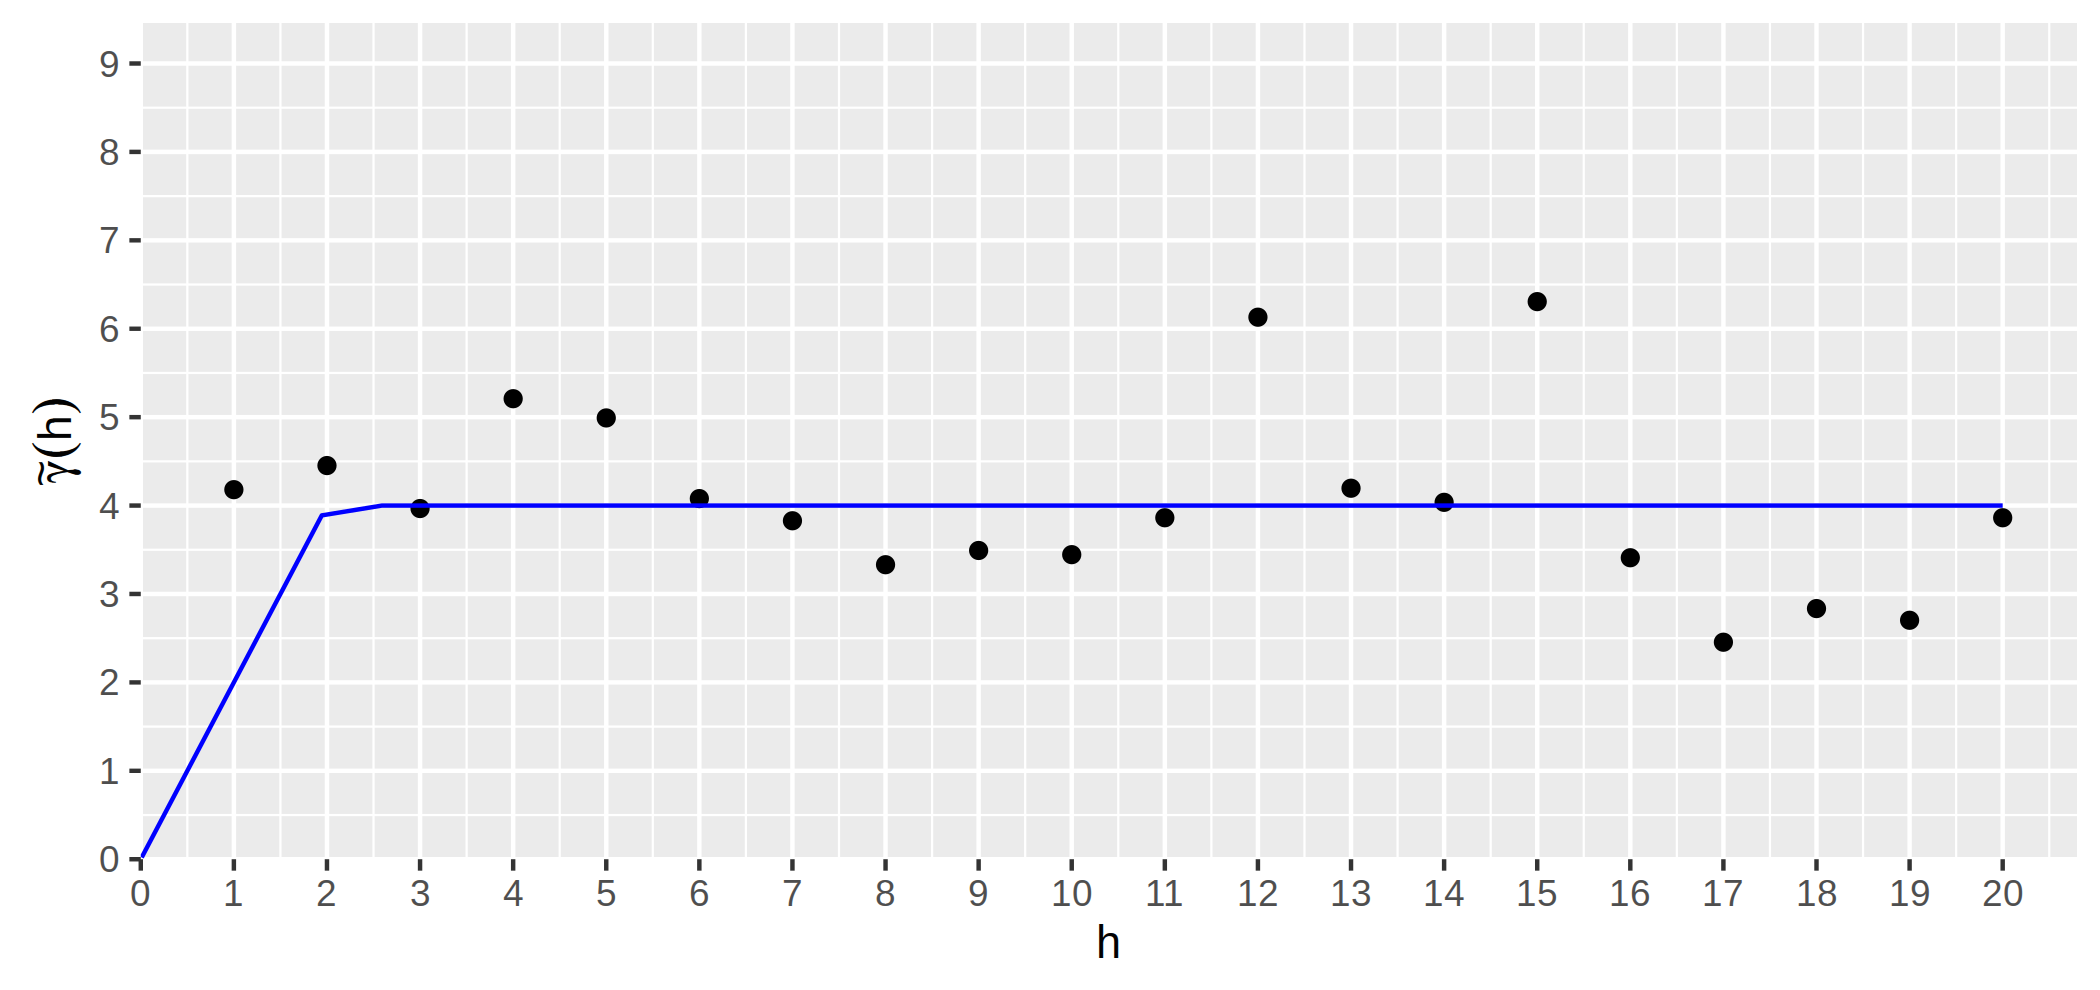
\includegraphics[width=1\linewidth]{../../figures/variogram/lin-fit-adapt-modeled.png} \\ Модель семивариограммы $\widehat{\gamma}_4(h)$
          \end{center}
        \end{minipage}
        \\
        \begin{minipage}[H]{0.95\linewidth}
          \begin{center}
            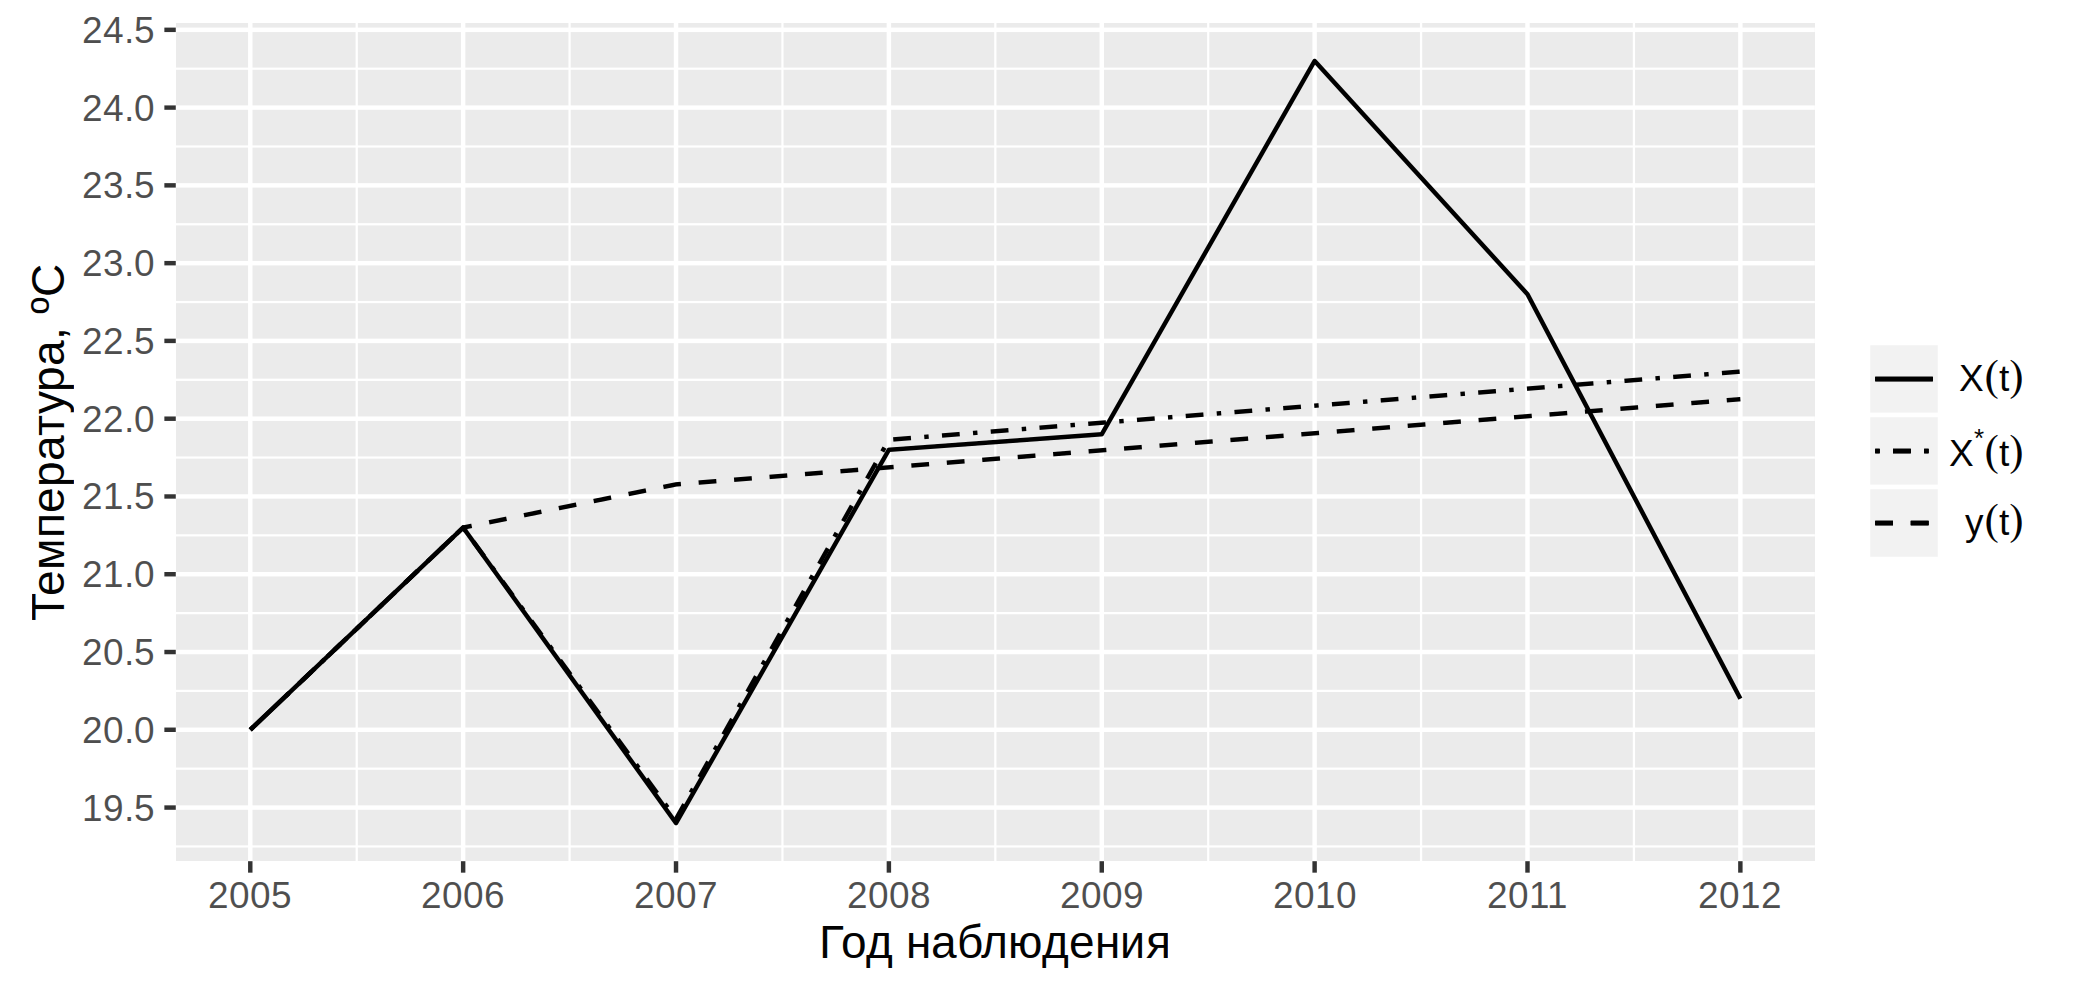
\includegraphics[width=1\linewidth]{../../figures/variogram/lin-fit-adapt-cross-prediction.png} \\ Прогноз по модели $\widehat{\gamma}_4(h)$
          \end{center}
        \end{minipage}
      \end{center}
    \end{figure}
  \end{multicols}
\end{frame}

\begin{frame}
  \frametitle{Вариограммный анализ}
  \framesubtitle{Сферическая модель}
  \begin{multicols}{2}
    \begin{small}
      Общий вид модели:
      \begin{equation}\begin{gathered}
      \label{eq:sph}
        \widehat{\gamma}(h) = c_0 + c \cdot Sph(h, a) = \\ = \left\{
        \begin{array}{l l}
          c_0 + c \cdot (\frac{3}{2} \frac{h}{a} - \frac{1}{2}(\frac{h}{a})^3), & h \le a, \\
          c_0 + c, & h \geq a,
        \end{array} \right.
      \end{gathered}\end{equation}
      где $ c_0 $ -- эффект самородков, $ c $ -- порог, $ a $ -- ранг.
      
      \medskip
      
      Подобранная модель:
      \begin{equation}
        \label{eq:gamma5}
        \widehat{\gamma}_5(h) = 0.9 + 4 Sph(h, 6.9),
      \end{equation}
      
      Показатели качества
      \begin{equation*}
        r_{\varepsilon\varepsilon^{*}} = -0.009, \quad MSE = 5.396
      \end{equation*}
    \end{small}
    
    \columnbreak
    \begin{figure}[H]
      \begin{center}
        \begin{minipage}[H]{0.95\linewidth}
          \begin{center}
            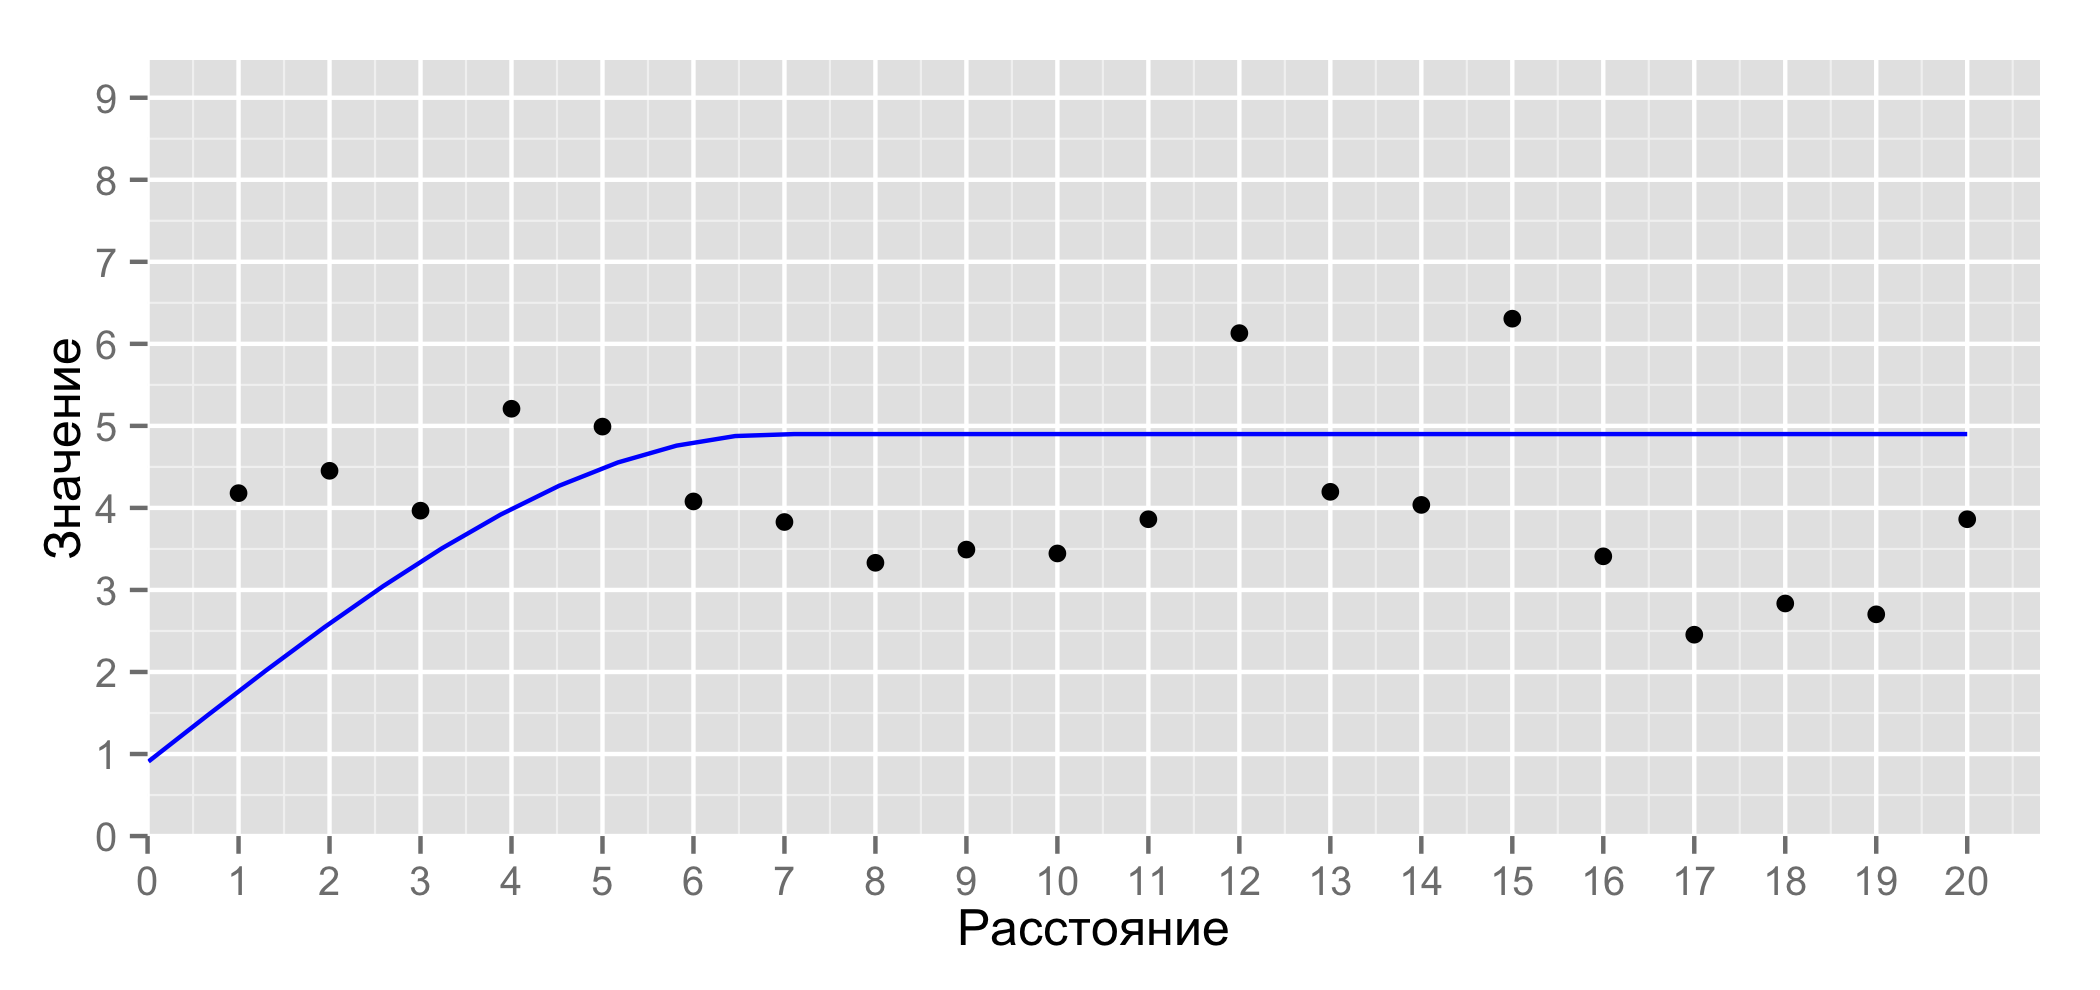
\includegraphics[width=1\linewidth]{../../figures/variogram/sph-fit-adapt-modeled.png} \\ Модель семивариограммы $\widehat{\gamma}_5(h)$
          \end{center}
        \end{minipage}
        \\
        \begin{minipage}[H]{0.95\linewidth}
          \begin{center}
            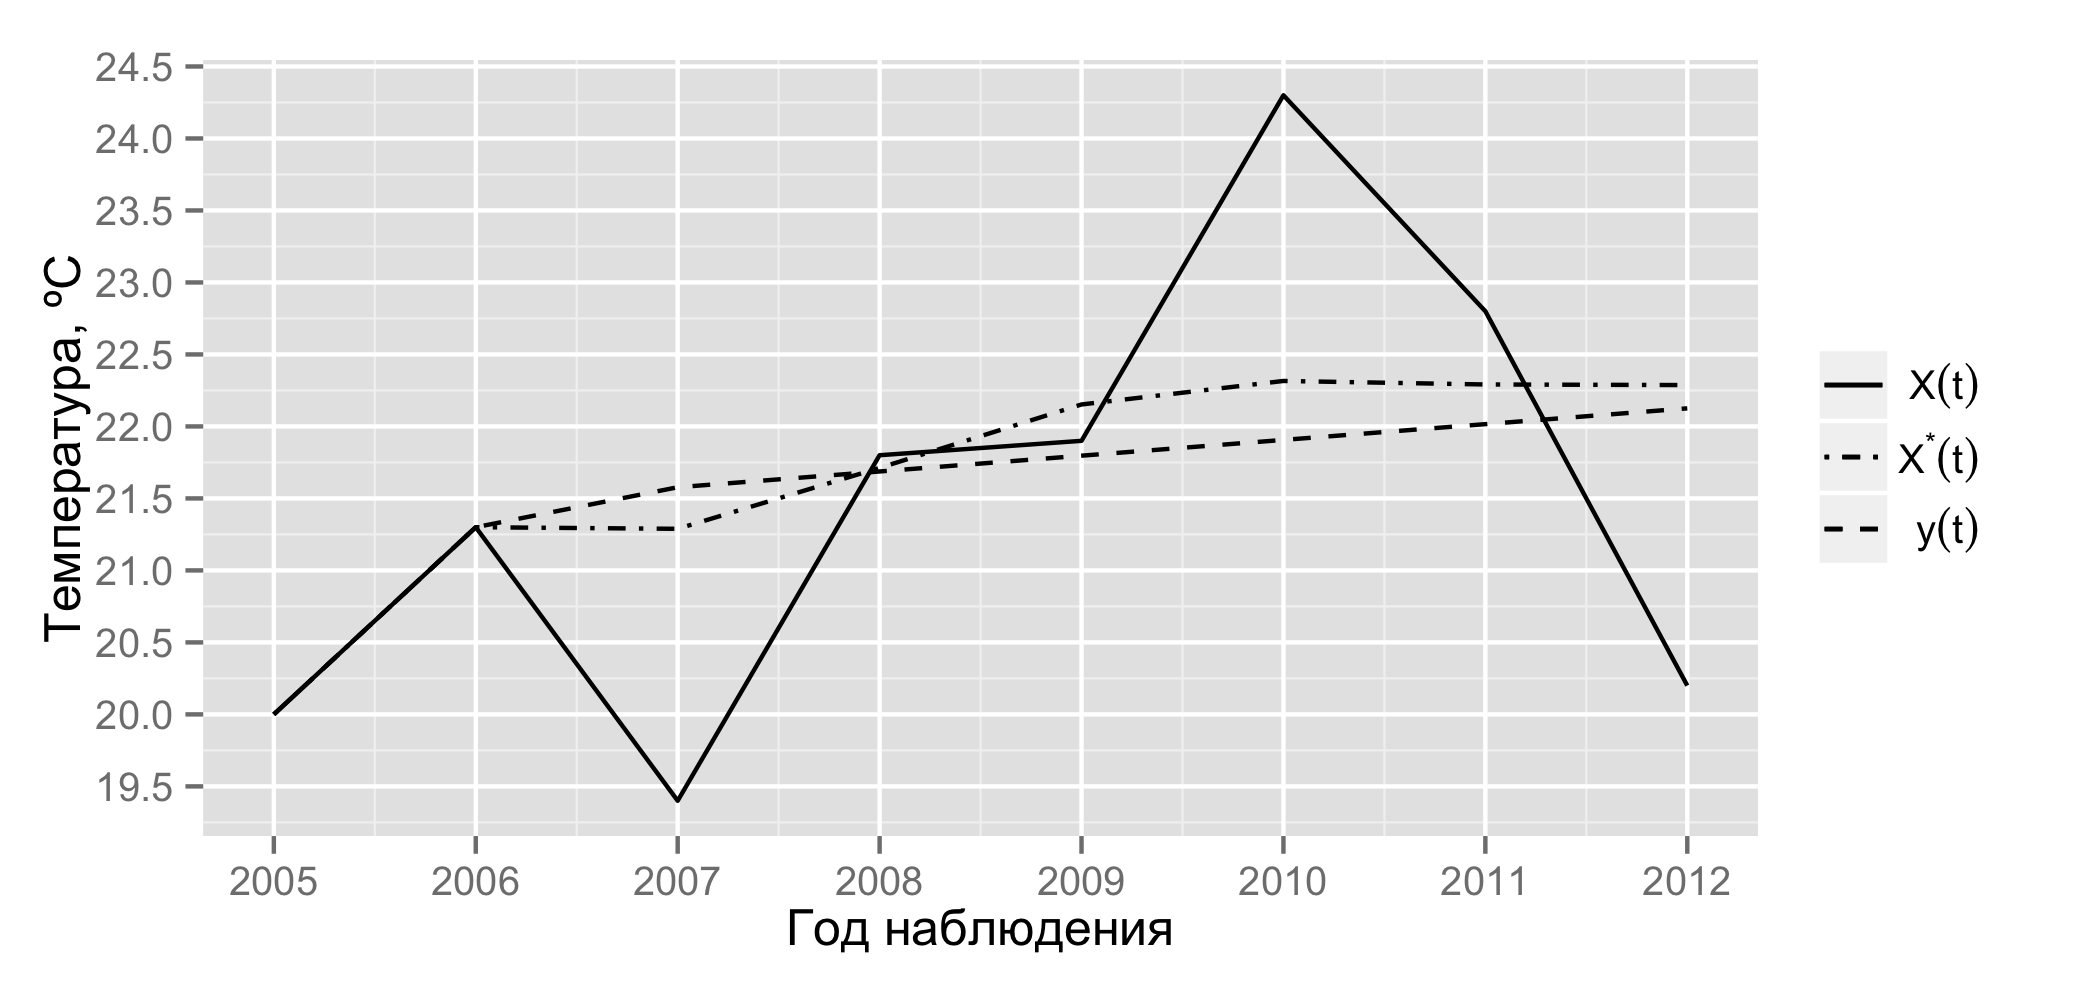
\includegraphics[width=1\linewidth]{../../figures/variogram/sph-fit-adapt-cross-prediction.png} \\ Прогноз по модели $\widehat{\gamma}_5(h)$
          \end{center}
        \end{minipage}
      \end{center}
    \end{figure}
  \end{multicols}
\end{frame}

\begin{frame}
  \frametitle{Вариограммный анализ}
  \framesubtitle{Периодическая модель}
  \begin{multicols}{2}
    \begin{small}
      Общий вид модели:
      \begin{eqnarray}
      \label{eq:per}
        \widehat{\gamma}(h) = c_0 + c \cdot Per(h, a) = \\ = 1 - cos(\frac{2 \pi h}{a}), \nonumber
      \end{eqnarray}
      где $ c_0 $ -- эффект самородков, $ c $ -- порог, $ a $ -- ранг.
      
      \medskip
      
      Подобранная модель:
      \begin{equation}
      \label{eq:gamma6}
        \widehat{\gamma}_6(h) = 4 \cdot Per(h, 0.898),
      \end{equation}
      
      Показатели качества
      \begin{equation*}
        r_{\varepsilon\varepsilon^{*}} = 0.404, \quad MSE = 4.369
      \end{equation*}
    \end{small}
    
    \columnbreak
    \begin{figure}[H]
      \begin{center}
        \begin{minipage}[H]{0.95\linewidth}
          \begin{center}
            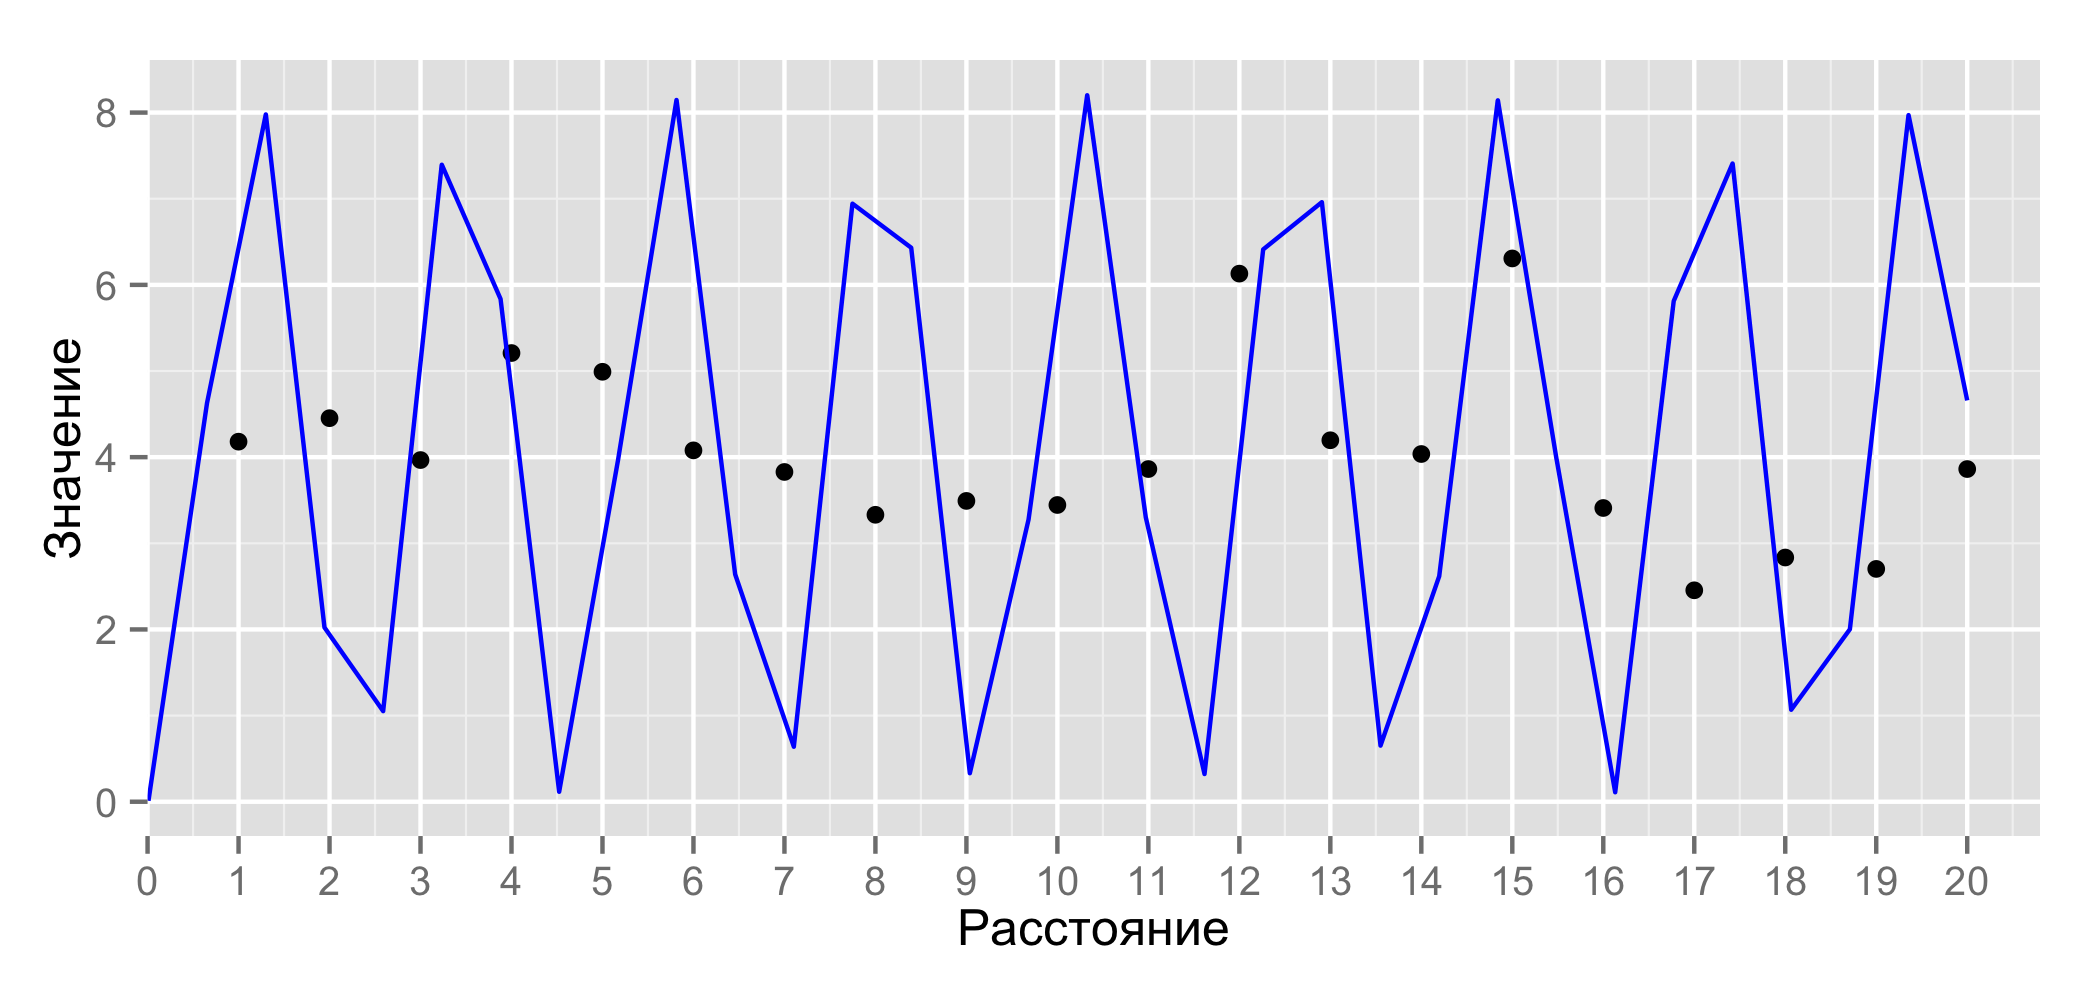
\includegraphics[width=1\linewidth]{../../figures/variogram/per-fit-cv-modeled.png} \\ Модель семивариограммы $\widehat{\gamma}_6(h)$
          \end{center}
        \end{minipage}
        \\
        \begin{minipage}[H]{0.95\linewidth}
          \begin{center}
            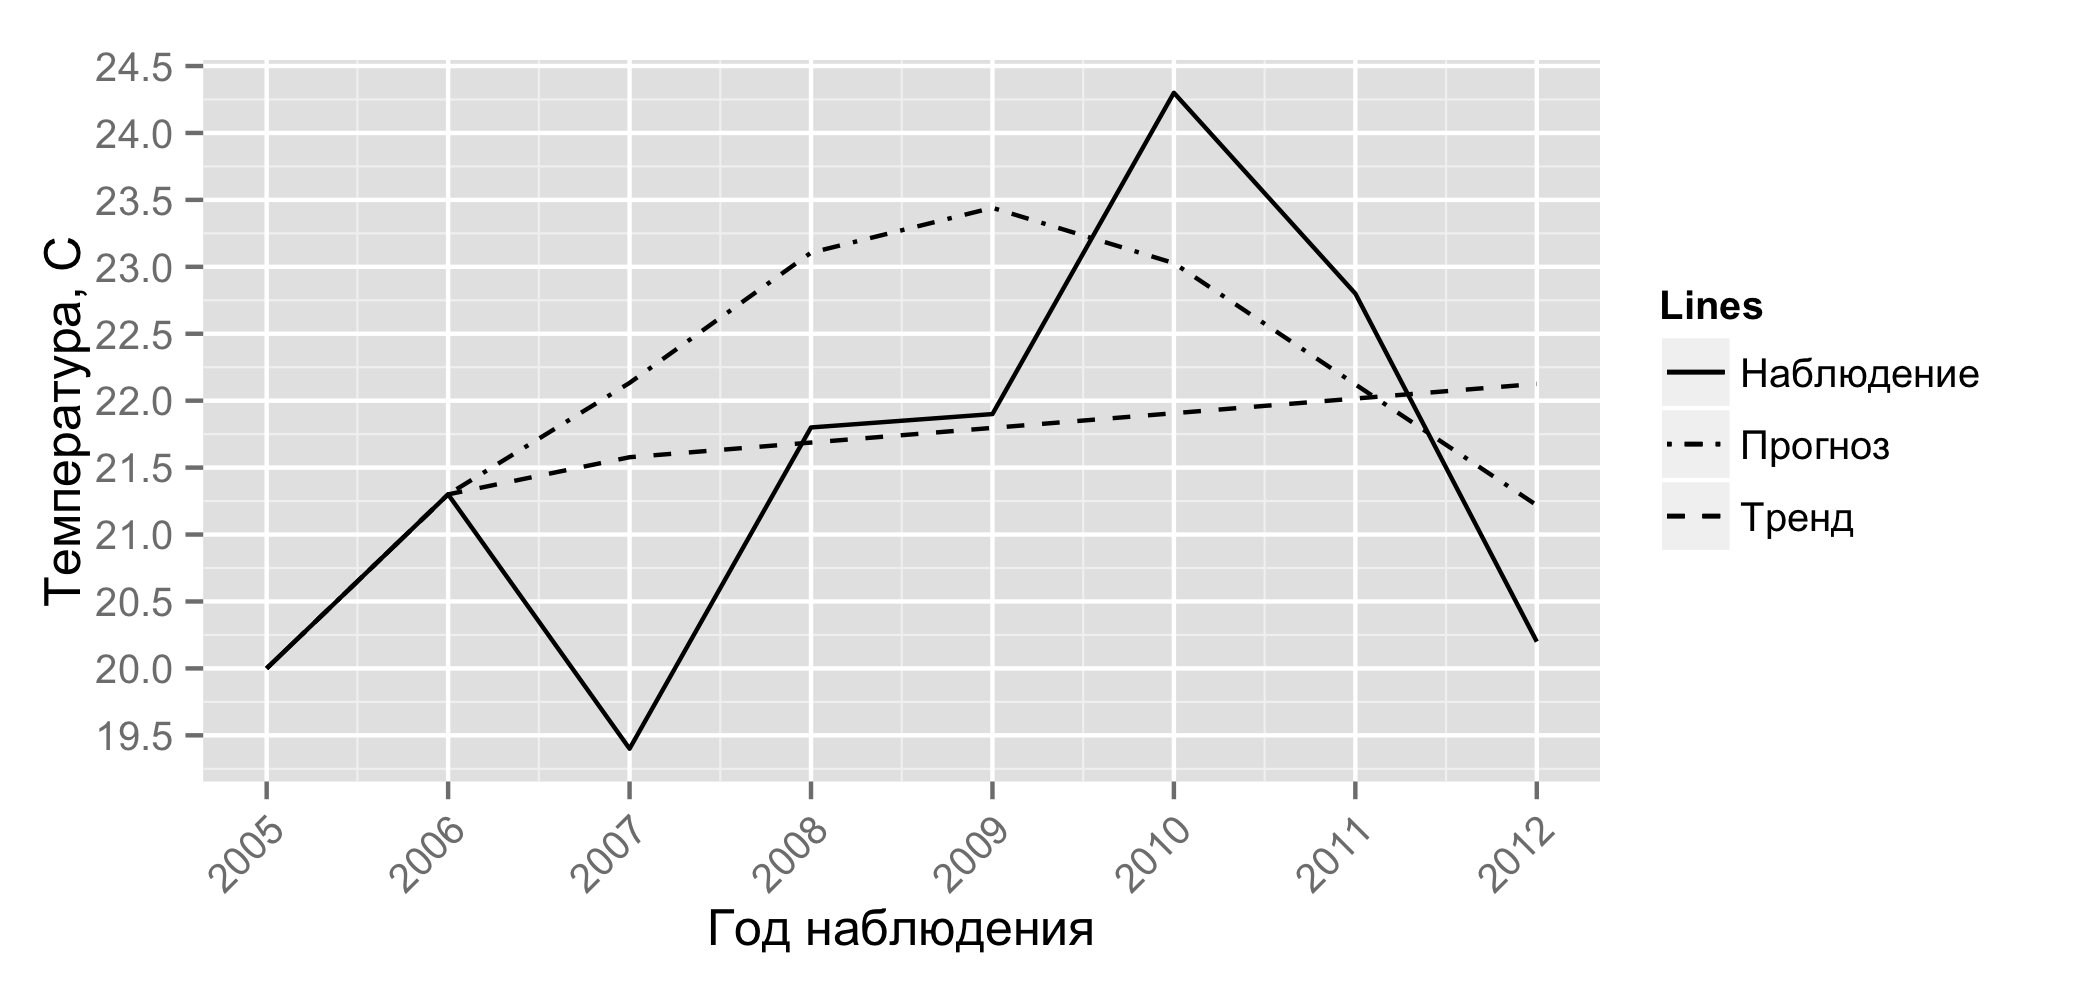
\includegraphics[width=1\linewidth]{../../figures/variogram/per-fit-cv-cross-prediction.png} \\ Прогноз по модели $\widehat{\gamma}_6(h)$
          \end{center}
        \end{minipage}
      \end{center}
    \end{figure}
  \end{multicols}
\end{frame}

\subsection{Автоматический подход}
\begin{frame}
  \frametitle{Автоматический подход}
  \framesubtitle{Волновая модель}
  \begin{multicols}{2}
    \begin{small}
      Общий вид модели:
      \begin{eqnarray}
      \label{eq:wave}
        \widehat{\gamma}(h) = c_0 + c \cdot Wav(h, a) = \\ = 1 - \frac{a}{h} \cdot sin(\frac{h}{a}), \nonumber
      \end{eqnarray}
      где $ c_0 $ -- эффект самородков, $ c $ -- порог, $ a $ -- ранг.
      
      \medskip
      
      Подобранная модель:
      \begin{equation}
      \label{eq:gamma9}
        \widehat{\gamma}_9(h) = 4.11 + 1.65 \cdot Wav(h, 3.59),
      \end{equation}
      
      Показатели качества
      \begin{equation*}
        r_{\varepsilon\varepsilon^{*}} = -1, \quad MSE = 4.20
      \end{equation*}
    \end{small}
    
    \columnbreak
    \begin{figure}[H]
      \begin{center}
        \begin{minipage}[H]{0.95\linewidth}
          \begin{center}
            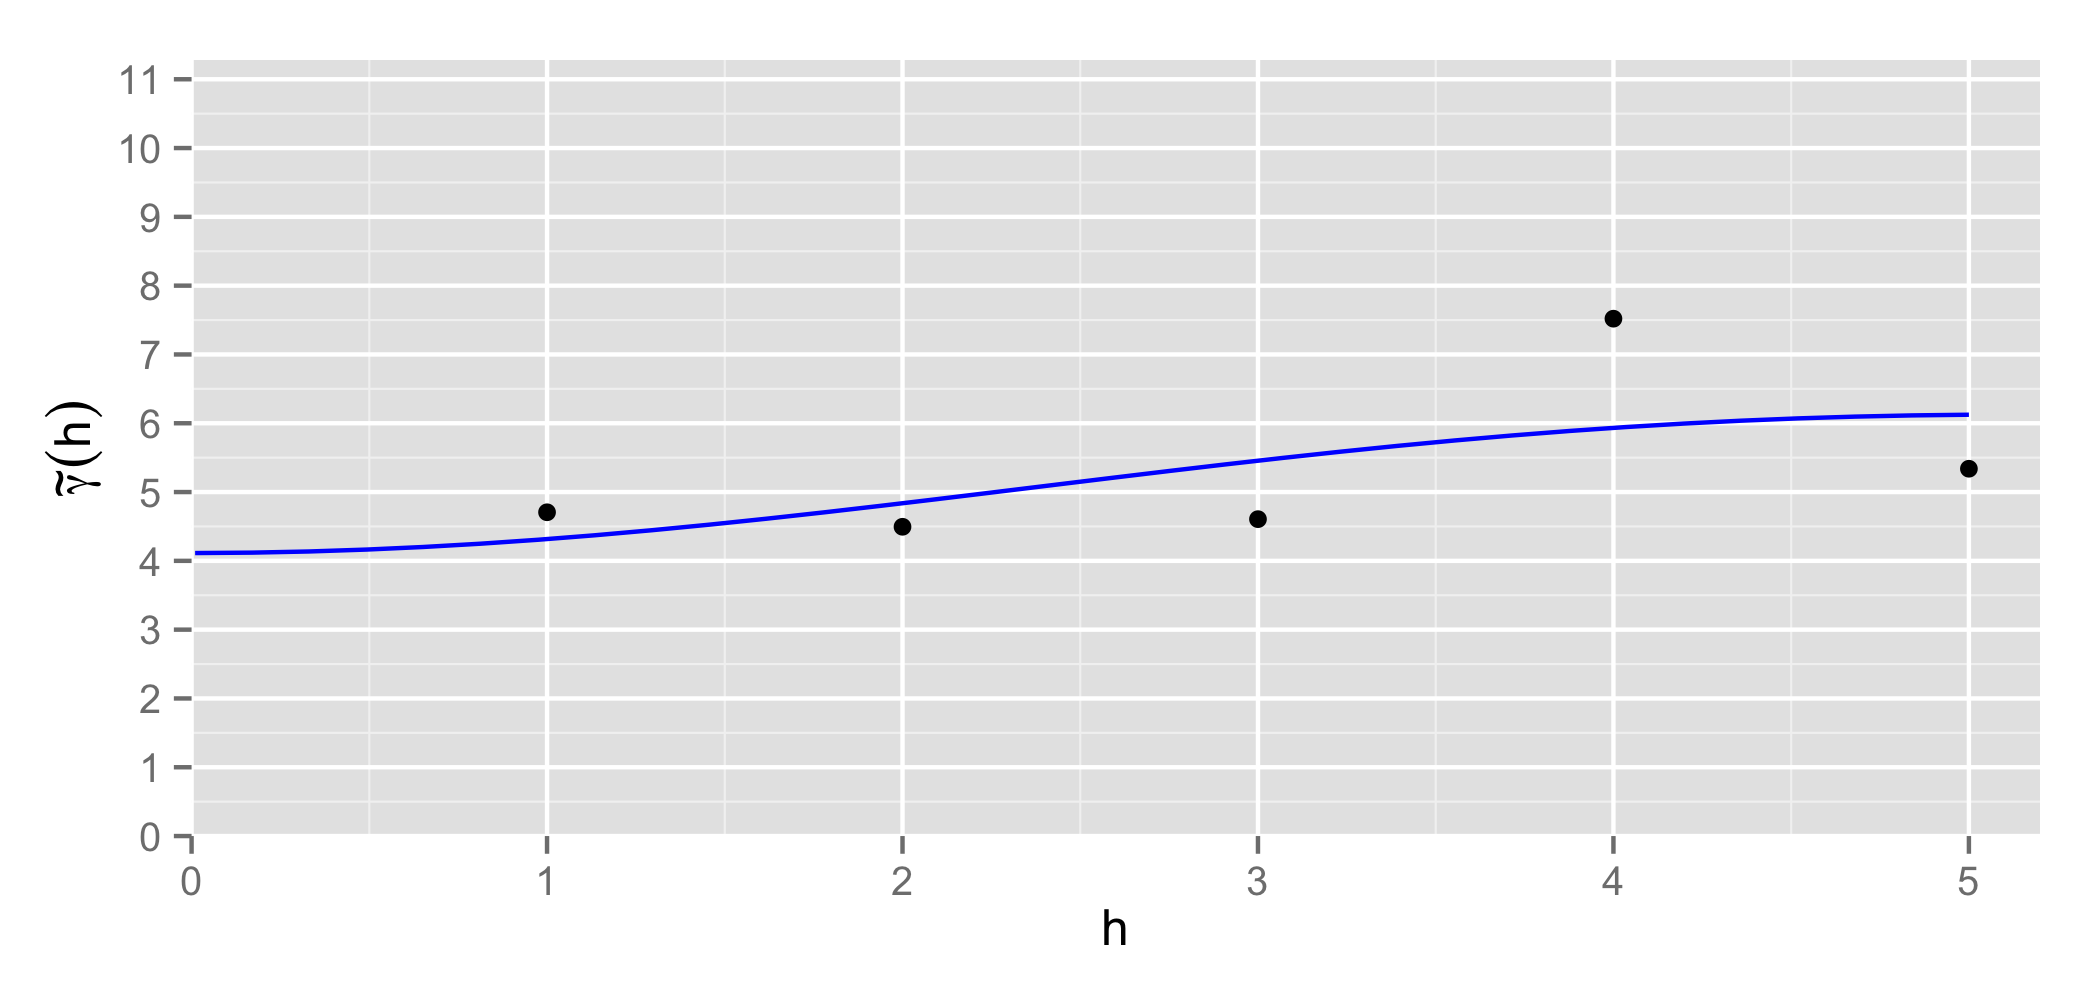
\includegraphics[width=1\linewidth]{../../figures/variogram/auto-rob-5-modeled.png} \\ Модель семивариограммы $\widehat{\gamma}_9(h)$
          \end{center}
        \end{minipage}
        \\
        \begin{minipage}[H]{0.95\linewidth}
          \begin{center}
            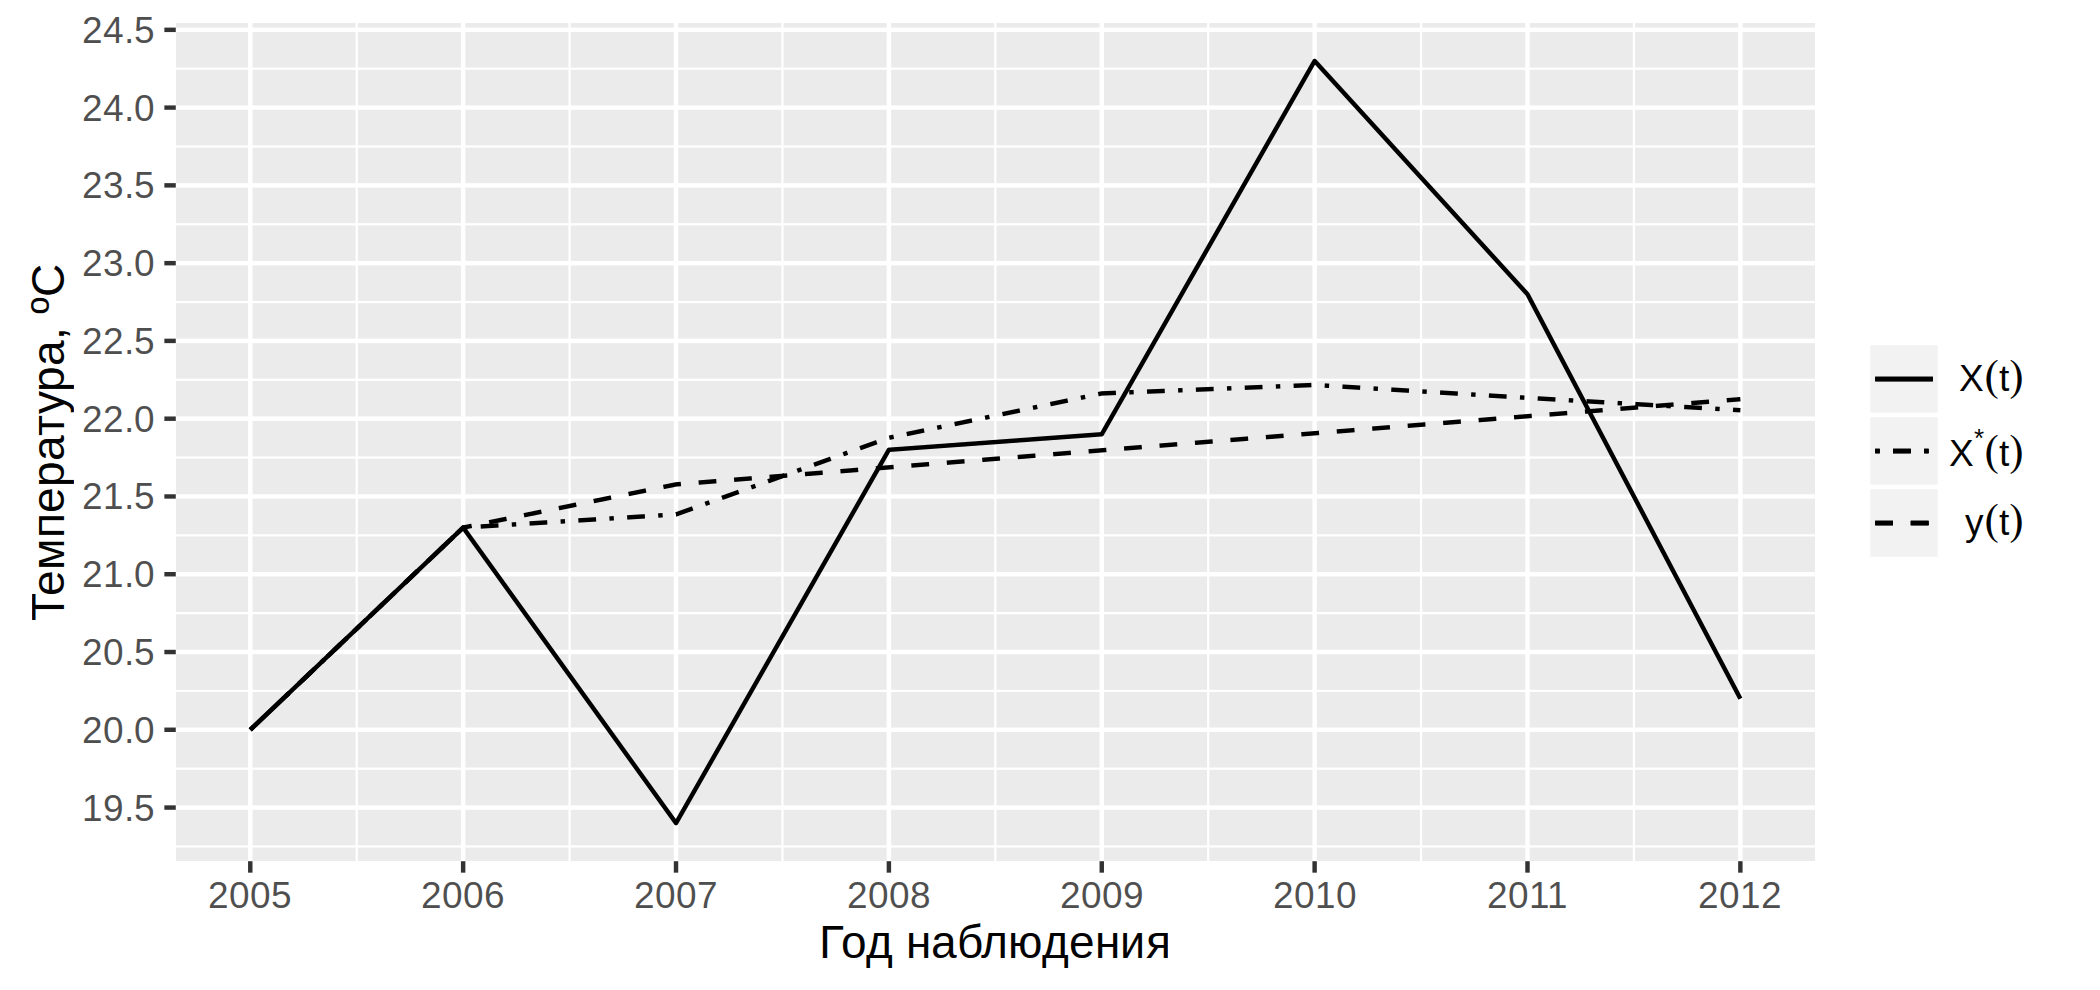
\includegraphics[width=1\linewidth]{../../figures/variogram/auto-rob-5-cross-prediction.png} \\ Прогноз по модели $\widehat{\gamma}_9(h)$
          \end{center}
        \end{minipage}
      \end{center}
    \end{figure}
  \end{multicols}
\end{frame}

\begin{frame}
  \frametitle{Автоматический подход}
  \framesubtitle{Периодическая модель}
  \begin{multicols}{2}
    \begin{small}
      Модель семивариограммы вида \eqref{eq:per}.
      
      \medskip
      
      Подобранная модель:
      \begin{equation}
        \label{eq:gamma10}
        \widehat{\gamma}_{10}(h) = 3.8 + 0.32 \cdot Per(h, 1.3)
      \end{equation}
      
      Показатели качества
      \begin{equation*}
        r_{\varepsilon\varepsilon^{*}} = -0.15, \quad MSE = 5.22
      \end{equation*}
    \end{small}
    
    \columnbreak
    \begin{figure}[H]
      \begin{center}
        \begin{minipage}[H]{0.95\linewidth}
          \begin{center}
            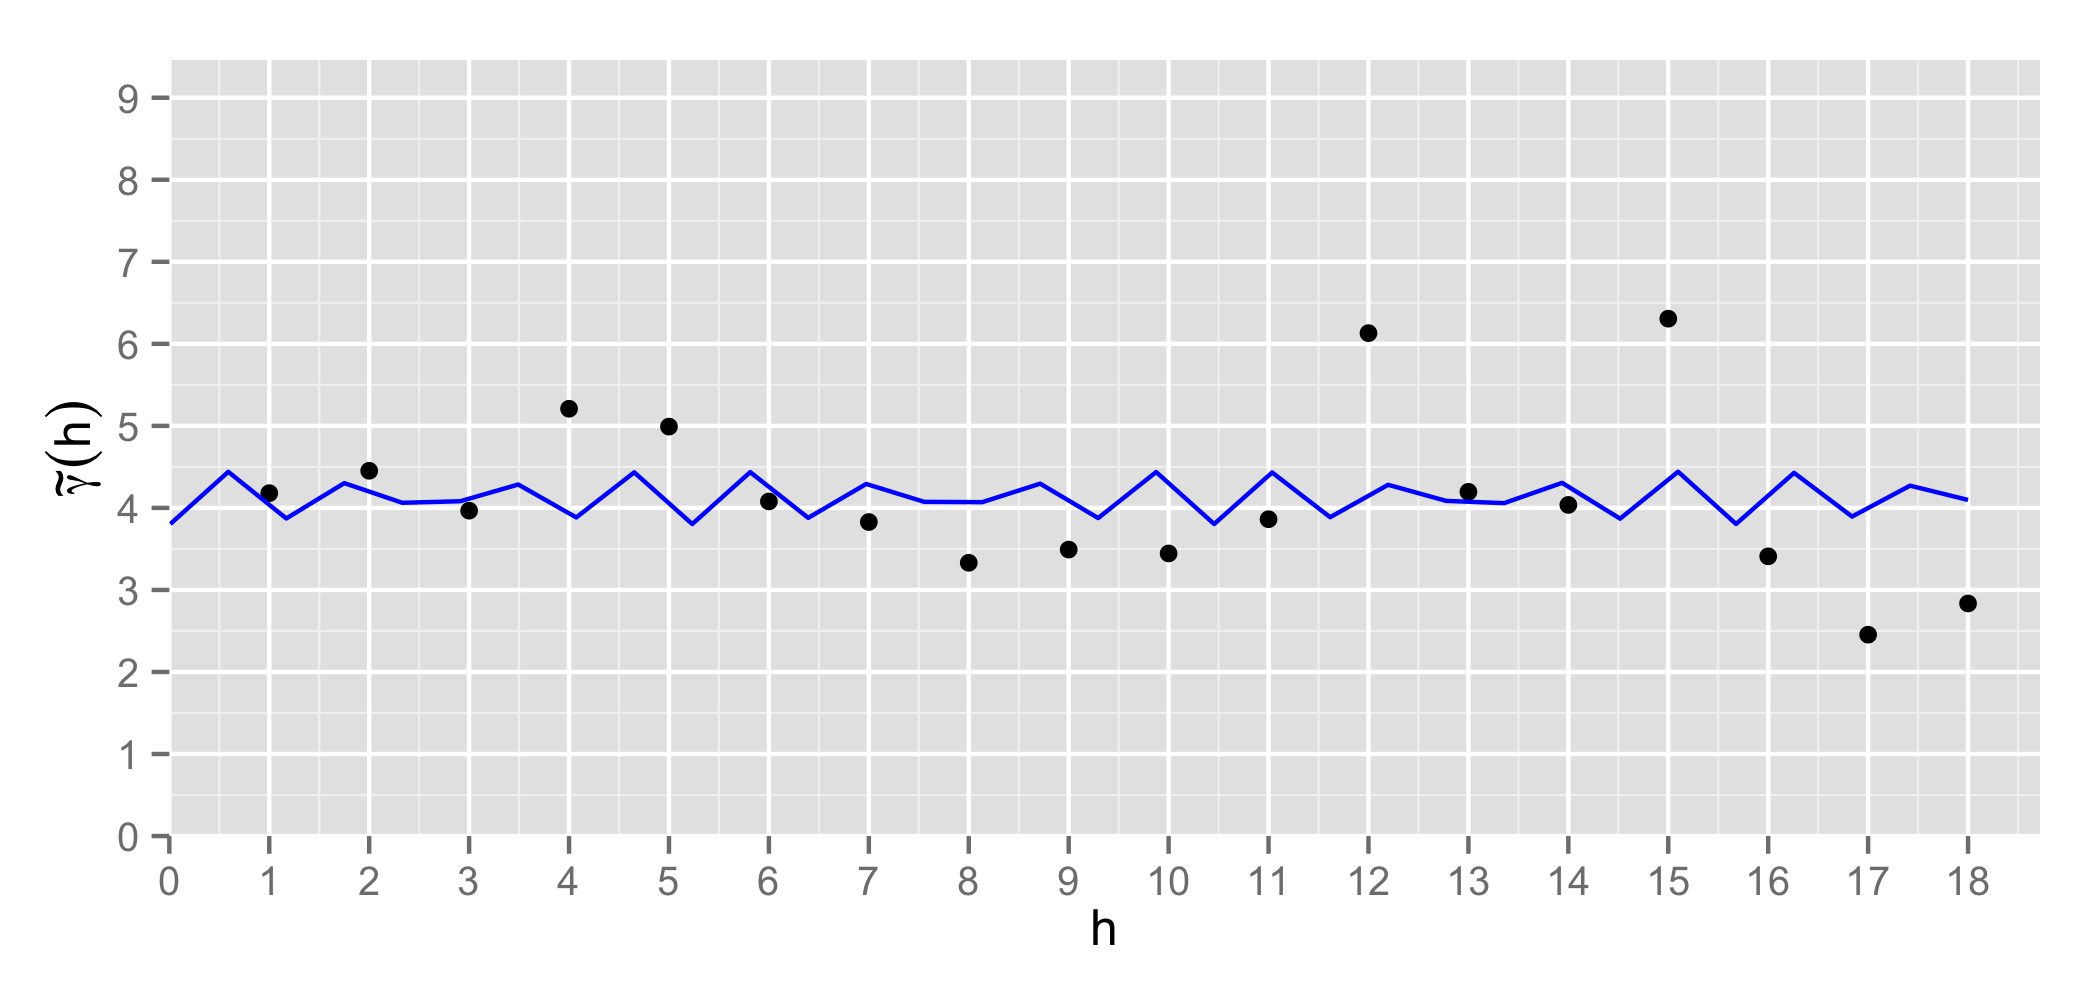
\includegraphics[width=1\linewidth]{../../figures/variogram/auto-class-18-modeled.png} \\ Модель семивариограммы $\widehat{\gamma}_{10}(h)$
          \end{center}
        \end{minipage}
        \\
        \begin{minipage}[H]{0.95\linewidth}
          \begin{center}
            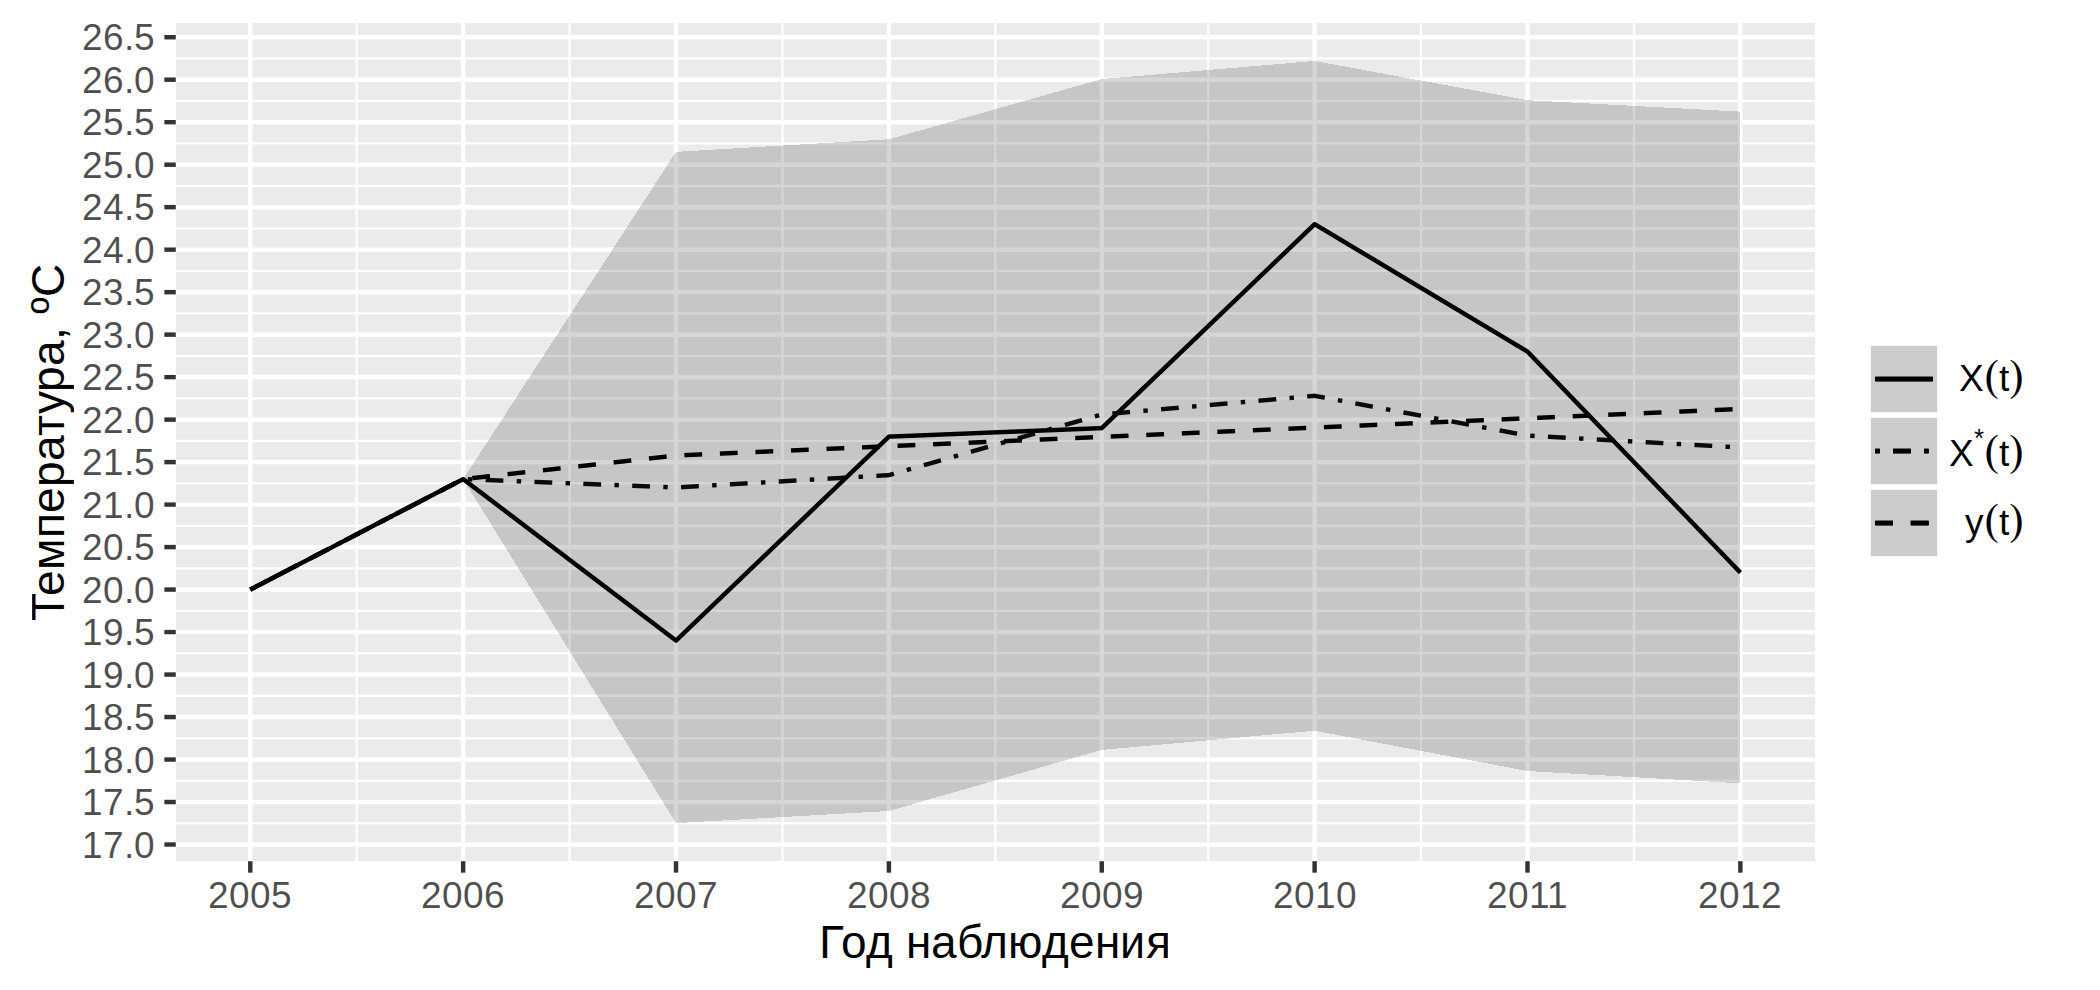
\includegraphics[width=1\linewidth]{../../figures/variogram/auto-class-18-cross-prediction.png} \\ Прогноз по модели $\widehat{\gamma}_{10}(h)$
          \end{center}
        \end{minipage}
      \end{center}
    \end{figure}
  \end{multicols}
\end{frame}

\section{Заключение}
\begin{frame}
  \frametitle{Заключение}
  \begin{itemize}
    \item Проведён предварительный статистический анализ данных:
      \begin{itemize}
        \item показана близость выборочного распределения к нормальному \normaldistr;
        \item показана умеренная положительная зависимость температуры от времени;
        \item построена регрессионная модель и вычислен ряд остатков;
      \end{itemize}
    \item Выполнен вариограммный анализ:
      \begin{itemize}
        \item рассмотрены два подхода по подбору моделей семивариограмм;
        \item визуальным подходом построены наилучшие модели: линейная модель с порогом \eqref{eq:gamma4} и периодическая \eqref{eq:gamma6};
        \item автоматическим подходом построены модели: волновая \eqref{eq:gamma9} и периодическая \eqref{eq:gamma10};
      \end{itemize}
  \end{itemize}
\end{frame}

\begin{frame}
  \frametitle{Заключение (продолжение)}
  \begin{itemize}
    \item По различным моделям построены прогнозные значения методом Кригинг. Проанализирована зависимость точности прогноза от оценки вариограммы и модели;
    \item Исследованы статистические свойства оценки семивариограммы гауссовского случайного процесса. Показана несмещённость и состоятельность в среднеквадратическом смысле оценки вариограммы \eqref{eq:matheron};
    \item Реализовано программное обеспечение, позволяющее решать класс задач, аналогичных исходной.
  \end{itemize}
\end{frame}

\begin{frame}
  \frametitle{Список использованных источников}
  \begin{scriptsize}
  \begin{thebibliography}{5}
    \beamertemplatebookbibitems
    \bibitem{cressie}
      Cressie~N.
      \newblock {\em Statistics for Spatial Data}.
      \newblock New York. --- Wiley, 1991.
    \beamertemplatebookbibitems
    \bibitem{saveliev}
      А.А.~Савельев, С.С.~Мухарамова, А.Г.~Пилюгин, Н.А.~Чижикова
      \newblock {\em Геостатистический анализ данных в экологии и природопользовании (с применением пакета R)}
      \newblock Казань: Казанский университет, 2012.
    \beamertemplatebookbibitems
    \bibitem{shumway}
      Robert H.~Shumway, David S.~Stoffer
      \newblock {\em Time series and Its Applications: With R Examples (Springer Texts in Statistics)}.
      \newblock Springer Science+Business Media, LLC 2011, 3d edition, 2011.
    \beamertemplatebookbibitems
    \bibitem{cook}
      Paul~Teetor
      \newblock {\em R Cookbook (O’Reilly Cookbooks))}.
      \newblock O’Reilly Media, 1 edition, 2011.
  \end{thebibliography}
\end{scriptsize}
\end{frame}

%\begin{frame}
%\frametitle{Блоки}
%	\begin{theorem}[Пифагора]
%		Если $a$ и $b$ "--- длины катетов прямоугольного треугольника, а~$c$ "--- длина гипотенузы, то $a^2+b^2=c^2$.
%	\end{theorem}
%
%	\begin{alertblock}{Блок с красным заголовком}
%		Содержимое.
%	\end{alertblock}
%
%	\begin{exampleblock}{Блок с зеленым заголовком}
%		Содержимое.
%	\end{exampleblock}
%\end{frame}

\begin{frame}[c]
\begin{center}
\frametitle{\LARGE Спасибо за внимание!}

{\LARGE \inserttitle}

\bigskip

{\insertauthor} 

\bigskip\bigskip

{\insertinstitute}

\bigskip\bigskip

{\large \insertdate}
\end{center}
\end{frame}

\end{document}